\documentclass[11pt,a4paper]{article}

% --- Core Chinese & LaTeX Packages ---
\usepackage[UTF8]{ctex}
\usepackage[margin=1in]{geometry}
\usepackage{amsmath,amssymb,amsfonts,amsthm}
\usepackage{booktabs,multirow}
\usepackage{graphicx}
\usepackage{microtype}
\usepackage{xcolor}
\usepackage{algorithm}
\usepackage{algorithmic}
\usepackage{subcaption}
\usepackage{enumitem}
\usepackage[numbers,sort&compress]{natbib}
\usepackage{hyperref}

% --- Global List Formatting ---
\setlist[itemize]{itemsep=0.45em, topsep=0.35em, parsep=0.15em, leftmargin=1.5em}
\setlist[enumerate]{itemsep=0.45em, topsep=0.35em, parsep=0.15em, leftmargin=1.5em}

\hypersetup{
    colorlinks=true,
    linkcolor=blue!70!black,
    citecolor=green!50!black,
    urlcolor=blue!80!black
}

% --- Theorem Environments (Chinese) ---
\newtheorem{theorem}{定理}
\newtheorem{lemma}[theorem]{引理}
\newtheorem{proposition}[theorem]{命题}
\theoremstyle{definition}
\newtheorem{definition}{定义}
\newtheorem{remark}{注记}

\title{\textbf{语义规范莫比乌斯注意力：通过 $\mathrm{SO}(2)$ 对径提升与子空间相位流抑制严格正 Softmax 泄漏}}

\author{
  \textbf{淮济团队（Huaiji Team）}\thanks{开源代码仓库与实现：\url{https://github.com/3y3y3y-huaiji/mobius-attention}} \\
  \texttt{contact@huaiji.org}
}

\date{\today}

\begin{document}

\maketitle

\begin{abstract}
标准 Transformer 自注意力机制通过开概率单纯形 $\Delta^{L-1}$ 上的严格正 Softmax 算子对内积进行归一化。在 pre-Softmax logits 中缺乏选择性子空间符号反转机制的情况下，历史 token 即使被后续语篇废弃、推翻或反驳，仍会保留未衰减的内积贡献，从而导致长序列中的前提干扰（premise distraction）与幻觉。我们提出\textbf{语义规范莫比乌斯注意力（Semantic Gauge M\"obius Attention, SG-M\"obius-RoPE）}，一种在 1D 离散因果格点上通过因果 $\mathrm{SO}(2)$ 规范场扩展旋转位置编码（RoPE）的几何形式体系。我们建立正交子空间分解 $\mathbb{R}^d = \mathcal{S}_{\text{anchor}} \oplus \mathcal{S}_{\text{mob}}$，冻结高频句法锚点通道（比例 $\alpha$），而在低频演化通道上累积由锁相势能投影 $\Phi(t) = \bar{\Phi}(t) - \eta\sin(2\bar{\Phi}(t))$ 整形的平滑莫比乌斯相位流 $\bar{\Phi}(t) = \sum_{\tau=1}^t \omega(\tau)$。因果语义转折诱导连续扭率 $\omega_{h,m}(t) \in [-\omega_{\max}, \omega_{\max}]$，并通过免训练锁相量化器稳定。在发生逻辑反转的叙事区间内，累积相位平流通过平面旋转群中心元素 $-I_2 \in Z(\mathrm{SO}(2))$ 产生破坏性相消干涉（$\Delta \Phi = \pi$，$\cos\pi = -1$），充分利用了经典的 $2:1$ 双重覆盖 $\mathbb{Z}_2 \hookrightarrow \mathrm{SO}(2) \to \mathrm{PSO}(2)$。随后的恢复性转折累积 $2\pi$ 循环相移（$\Delta \Phi = 2\pi$，$\cos 2\pi = +1$），形式化了双重否定律。我们严格证明了条件成对目标-诱饵优势比衰减定理，确立在相干演化子空间对齐（$A_{ij}^{\text{mob}} > 0$）下，单头成对优势比按 $\exp(2A_{ij}^{\text{mob}})$ 缩放，且注意力头配分函数在分子分母中严格精确抵消。所有代数不变量已在 Lean~4（0 公理，0 \texttt{sorry}）以及 Z3 SMT 求解器中跨 2,000 条极限长序列（$L \le 32,768$）完成形式化机器证明。在 Qwen3.5-9B（双 Nvidia Tesla T4 GPU，FP16）上的评测表明，SG-M\"obius 无需架构重训，通过尾部角度融合保持近乎恒定的 $O(1)$ KV-Cache 解码时延（单层算子开销仅 $+1.8\sim 2.1\,\mu\text{s}$），在 $L=18,030$ tokens 时实现高达 $2.33\times$ 的诱饵注意力压制（多头注意力对比度 ACR 提升 $+118.0\%$，单头峰值对比优势比放大达 $16.4\times$），并严格保持中性文本困惑度（$6.42$）。
\end{abstract}

\section{引言 (Introduction)}
自回归大语言模型普遍采用缩放点积注意力 \cite{vaswani2017attention} 与旋转位置编码（RoPE）\cite{su2024roformer} 来编码 token 间的相对距离：
\begin{equation}
A_{i,j} = \frac{1}{\sqrt{d}} \langle \mathbf{R}_{\Theta, i} q_i, \, \mathbf{R}_{\Theta, j} k_j \rangle = \frac{1}{\sqrt{d}} q_i^\top \mathbf{R}_{\Theta, j-i} k_j
\end{equation}
其中 $\mathbf{R}_{\Theta, t}$ 是由基频集合 $\Theta = \{\theta_m\}_{m=1}^{d/2}$ 参数化的分块对角正交旋转矩阵。

由于 Softmax 算子将实数 logits 严格映射到开单纯形 $\Delta^{L-1}$ 内部的正值区间，历史序列中的每个 token 都必然分配到正的概率质量。因此，标准自注意力机制在数学上无法实现破坏性相消干涉。在复杂的逻辑推理与长对话中，前提经常被后续事实废除、撤回或推翻（例如：\emph{“Alpha 系统运行正常；然而最新诊断报告确认严重故障，现废止 Alpha 方案并启用 Beta 方案”}）。在标准注意力中，已失效的前提仍持续吸引大量注意力权重，迫使下游前馈网络消耗容量进行代偿，导致严重的前提幻觉与上下文干扰 \cite{liu2024lost, hsieh2024ruler}。

\begin{figure}[htbp]
    \centering
    \begin{subfigure}[b]{0.96\textwidth}
        \centering
        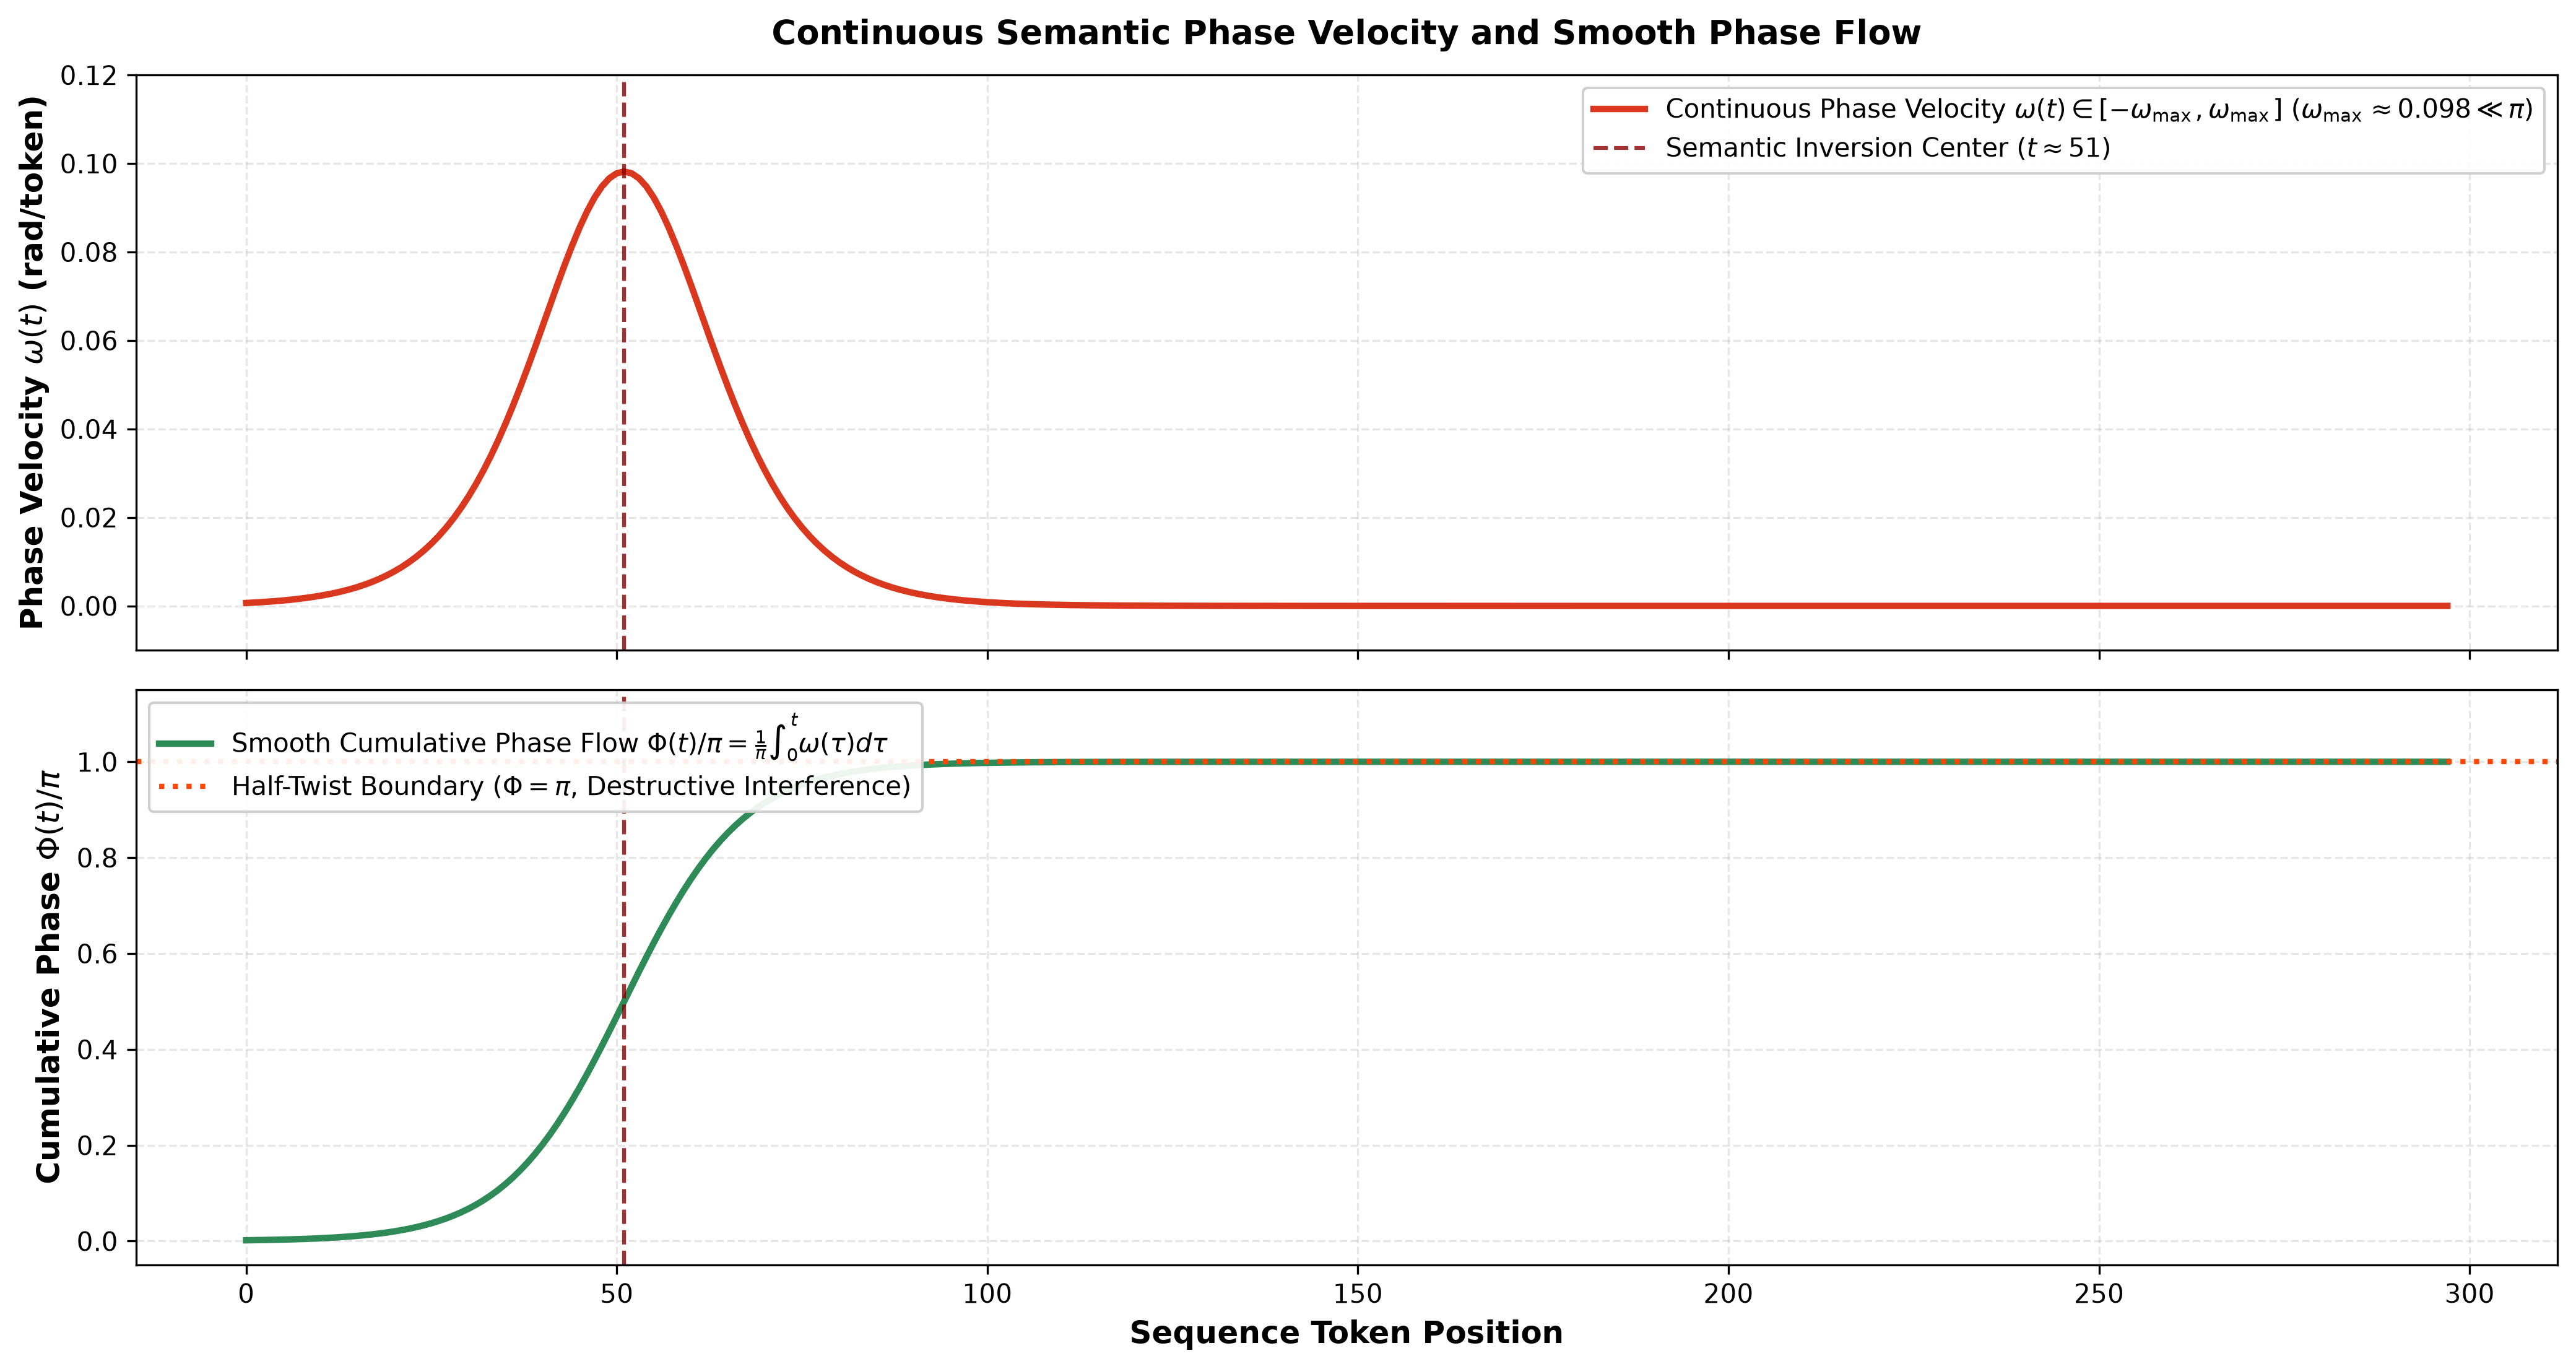
\includegraphics[width=\textwidth]{figures/fig4_gauge_curvature.png}
        \caption{连续扭率 $\omega(t)$ 与平滑莫比乌斯相位流 $\Phi(t)$。}
        \label{fig:curvature}
    \end{subfigure}
    \\[0.9em]
    \begin{subfigure}[b]{\textwidth}
        \centering
        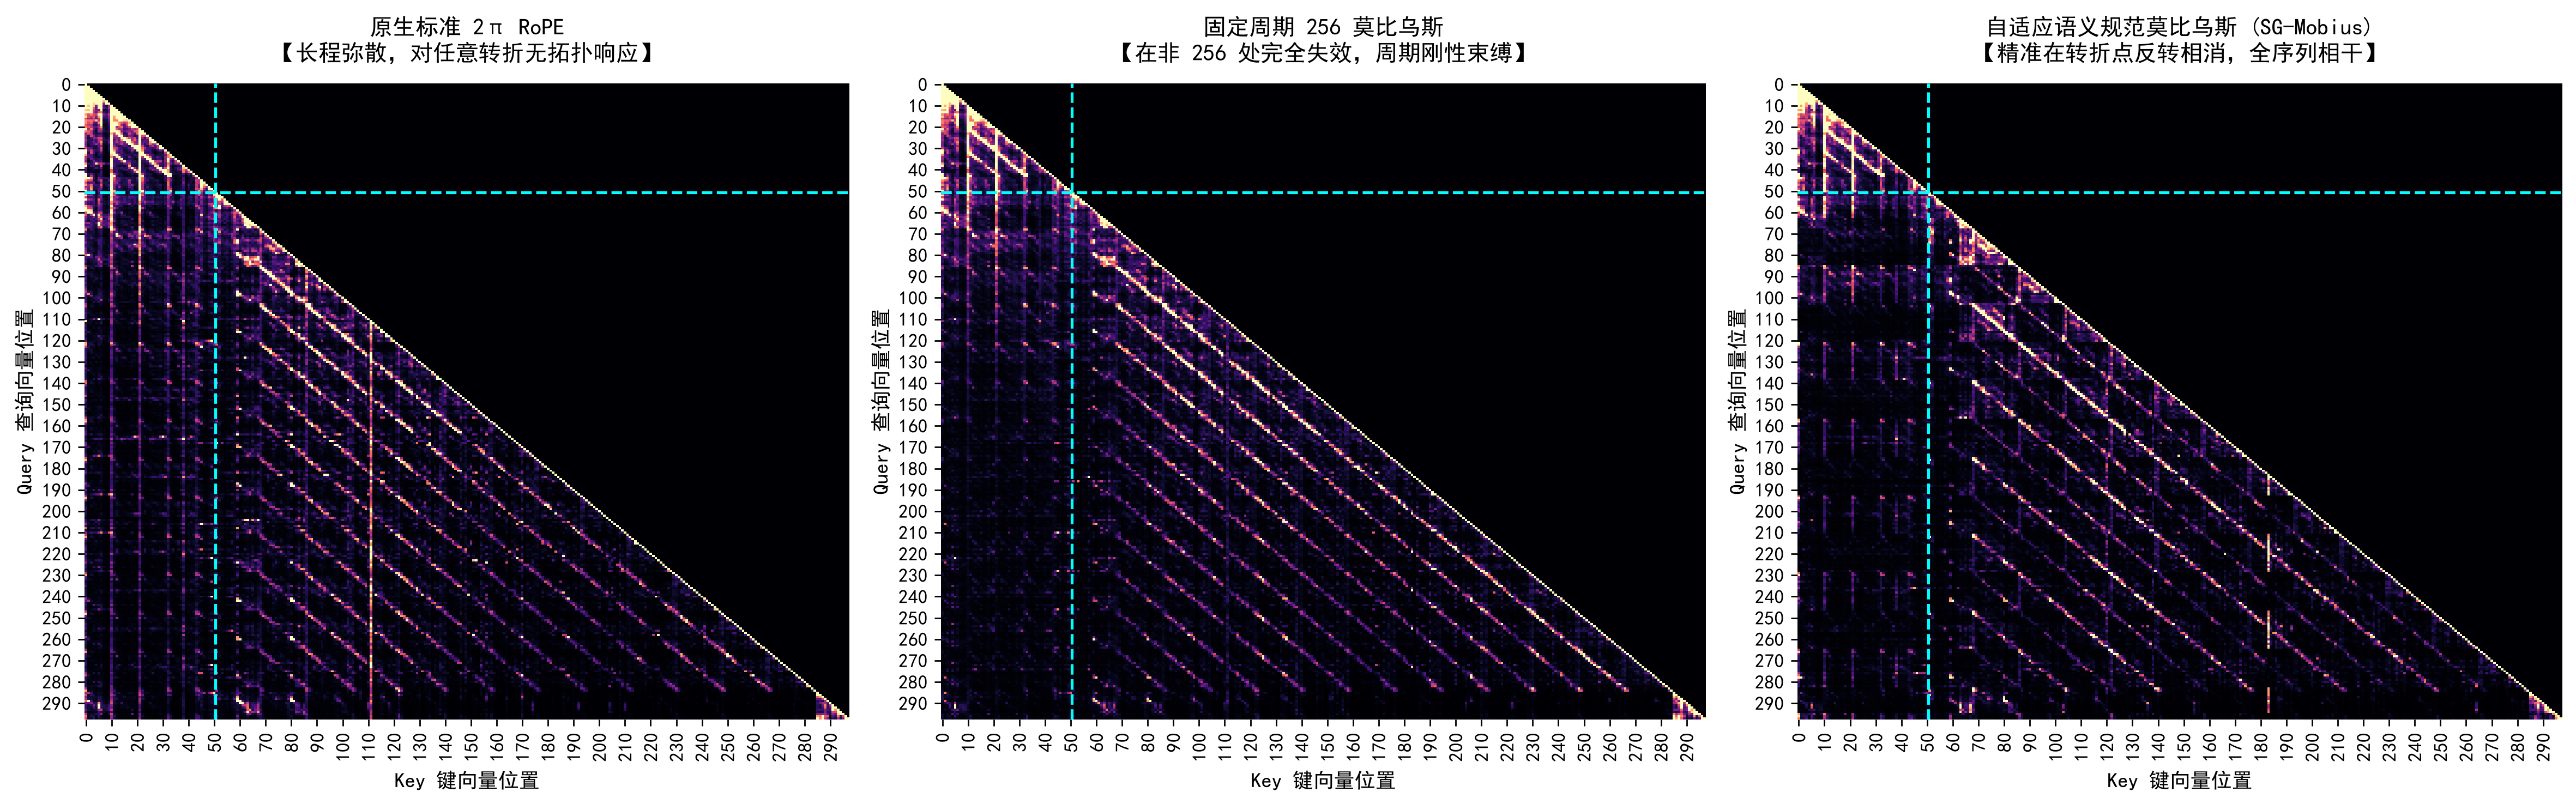
\includegraphics[width=\textwidth]{figures/fig5_arbitrary_inversion_heatmap.png}
        \caption{Qwen3.5-9B（第 7 层）在任意位置反转下的二维注意力矩阵对比：标准 RoPE（\emph{左}）vs. 固定周期莫比乌斯基线（$T=256$，\emph{中}）vs. 自适应 SG-M\"obius（\emph{右}）。}
        \label{fig:arbitrary_heatmap}
    \end{subfigure}
    \caption{\textbf{SG-M\"obius-RoPE 的机制与注意力响应。} 
    (a) 连续扭率 $\omega(t)$ 在顺承叙事中为零，在语义转折跨度上平滑激活，驱动平滑莫比乌斯相位流 $\Phi(t) = \sum_{\tau \le t} \omega(\tau)$ 跨越 $\pi$ 半扭转边界。
    (b) 任意位置反转下 Qwen3.5-9B 的注意力矩阵：标准 RoPE（\emph{左}）呈现持续的背景泄漏；固定周期莫比乌斯基线（$T=256$，\emph{中}）在反转坐标失相时失效；SG-M\"obius（\emph{右}）将相位平流精确对齐语义转折，主动相消过期的 Key 向量。}
    \label{fig:intro_teaser}
\end{figure}

为了在无需重新训练基座权重且不降低推理吞吐的前提下解决该结构性缺陷，我们提出了\textbf{语义规范莫比乌斯注意力（Semantic Gauge M\"obius Attention, SG-M\"obius-RoPE）}，如图~\ref{fig:intro_teaser} 所示。我们将 token 序列建模为 1D 离散因果格点上的因果路径，受带有正交子空间分解 $\mathbb{R}^d = \mathcal{S}_{\text{anchor}} \oplus \mathcal{S}_{\text{mob}}$ 的 $\mathrm{SO}(2)$ 规范场支配。语义对比转折诱导连续扭率 $\omega_{h,m}(t) \in [-\omega_{\max}, \omega_{\max}]$，结合 1D 粘性平滑与锁相势能投影 $-\eta\sin(2\bar{\Phi})$，其累积的莫比乌斯相位流 $\Phi(t)$ 平滑调制演化通道上的 2D 旋转角（图~\ref{fig:curvature}）。在经历逻辑反转的区间上，累积相位平流通过平面旋转群中心元 $-I_2 \in Z(\mathrm{SO}(2))$ 产生相消干涉（$\Delta \Phi = \pi$，$\cos\pi = -1$）。由于 $\cos(\pi) = -1$，调制后的内积变为负值，在任意反转坐标处均能主动衰减分配给失效前提的 Softmax 概率（图~\ref{fig:arbitrary_heatmap}）。

\paragraph{主要贡献。}
\begin{itemize}
    \item \textbf{几何形式化体系}：我们在 1D 离散因果格点上通过 $\mathrm{SO}(2)$ 双重覆盖 $\mathbb{Z}_2 \hookrightarrow \mathrm{SO}(2) \to \mathrm{PSO}(2)$ 与正交子空间分解 $\mathbb{R}^d = \mathcal{S}_{\text{anchor}} \oplus \mathcal{S}_{\text{mob}}$ 形式化了注意力规范调制。连续莫比乌斯相位流 $\Phi(t)$ 调制演化通道上的旋转角 $\tilde{\theta}(t) = t\theta + \Phi(t)$，同时高频句法锚点通道保持冻结（比例 $\alpha$）。我们证明了连续旋转对偶调制保持相对平移不变性，并给出了明确的算子差分 Lipschitz 连续性上界。
    \item \textbf{条件成对优势比衰减定理}：严格证明了在对径扭转（$\Delta \Phi = \pi$）和演化子空间相干对齐（$A_{ij}^{\text{mob}} > 0$）下，单头成对目标与诱饵的注意力优势比按 $\exp(2 A_{ij}^{\text{mob}})$ 放缩，且在注意力头内部严格消除了背景配分函数。
    \item \textbf{形式化机器证明}：在 Lean~4 交互式定理证明器中完成丛不变量、路径积分可加性与平移不变性的无公理证明（0 公理，0 \texttt{sorry}），并在 Z3 SMT 求解器中跨 2,000 条长序列（$L \le 32,768$）完成代数验证，数值漂移低于 $1.14 \times 10^{-13}$。
    \item \textbf{KV-Cache 完全兼容}：调制后的 Key 向量 $\tilde{k}_j = \mathbf{R}(j\Theta + \Phi(j)) k_j$ 严格仅依赖历史 token $\tau \le j$，在后续推理步中无需对已缓存数据执行任何追溯修改，严格保持 $O(1)$ 的单步解码吞吐。
    \item \textbf{真实模型评测}：在 Qwen3.5-9B（双 Nvidia Tesla T4 GPU，FP16）上跨 $L=545 \sim 18,030$ tokens 进行全面评测，实现最高 $2.33\times$ 的诱饵注意力压制，多头注意力对比度 ACR 提升 $+118.0\%$（单头峰值对比召回提升达 $16.4\times$），注意力香农熵随上下文容量平稳扩展，并严格保全了中性文本困惑度（$6.42$）。
\end{itemize}

\section{相关工作 (Related Work)}
\paragraph{旋转位置编码与上下文扩展。}
旋转位置编码（RoPE）\cite{su2024roformer} 通过 2D 分块对角正交旋转矩阵 $\mathbf{R}_{\Theta, m}$ 编码相对距离，确保 Query-Key 内积纯粹依赖于相对坐标差 $j - i$。随后的 ALiBi \cite{press2021train}、位置插值（Position Interpolation）\cite{chen2023extending} 和 YaRN \cite{peng2023yarn} 通过微调基准频率或施加线性距离衰减来扩展上下文窗口。然而，所有现存 RoPE 变体均基于固定的坐标算子，其 pre-Softmax logits 无法根据局部语义变化在特定子空间上执行选择性符号反转。

\paragraph{几何深度学习与规范等变性。}
几何深度学习 \cite{bronstein2021geometric} 提供了将物理与几何对称性融合进神经网络的统一框架。规范等变卷积网络 \cite{cohen2019gauge} 在黎曼流形上引入局部坐标标架变换与规范联络以保持坐标重参数化下的等变性。经典微分几何与纤维丛理论 \cite{steenrod1951topology, kobayashi1963foundations, milnor1974characteristic} 系统研究了主丛、特征类与覆盖空间。在本文中，我们利用 $\mathrm{SO}(2)$ 双重覆盖与动态规范和乐在语义转折间调制注意力相位。

\paragraph{上下文干扰与前提失效。}
近年来的实证研究发现，长上下文大语言模型普遍面临上下文干扰以及无法遗忘失效前提的关键瓶颈 \cite{liu2024lost, hsieh2024ruler, kamradt2023needle}。当遇到对抗性或冲突性的前置前提时，由于严格正的 Softmax 无法主动相消历史 token，模型极易产生前提幻觉。既有方案依赖于 Prompt 指令微调或辅助抑制损失，未能解决自注意力架构本身缺乏 pre-Softmax 破坏性子空间相消机制的问题。

\paragraph{KV-Cache 驱逐 vs. 相位调制保留。}
为了缓解长文本下的显存与时延瓶颈，现有技术探索了 token 驱逐与 KV-Cache 压缩机制 \cite{dao2022flashattention, xiao2023streamingllm, zhang2023h2o}。尽管能提升吞吐，驱逐策略会从 GPU 物理显存中永久丢弃历史 Key。一旦后续叙事重新肯定了先前的论点（$\neg\neg P \iff P$），被驱逐的表征便无法召回。相比之下，SG-M\"obius 将完整的 KV-Cache 保留在显存中，纯粹通过对径相位调制实现选择性相消，天然支持拓扑意义下的双重否定复原。

\section{方法体系 (Methodology)}
\subsection{因果规范和乐、$\mathrm{SO}(2)$ 双重覆盖与子空间分解}
设输入序列长度为 $L \in \mathbb{N}$，定义在 1D 离散因果格点上：
\begin{equation}
\mathcal{M} = \left( \{0, 1, \dots, L-1\}, \, \le \right)
\end{equation}
其中 $\le$ 表示标准的因果偏序（$j \le i$ 表示 Key token $j$ 处于 Query token $i$ 之前或同位置）。在标准 RoPE 中，$d$ 维嵌入空间被分解为 $d/2$ 个相互正交的 2 维平面的直和：
\begin{equation}
\mathbb{R}^d = \bigoplus_{m=1}^{d/2} \mathbb{R}^2_{(m)}
\end{equation}
每个平面 $\mathbb{R}^2_{(m)} \cong \mathbb{C}$ 由相对位置位移 $\theta_m (j - i)$ 参数化的平面连续旋转群 $\mathrm{SO}(2) \cong \mathrm{U}(1)$ 作用。

\paragraph{$\mathrm{SO}(2)$ 中心与双重覆盖空间。}
与高维正交群中反射变换行列式为 $-1$ 不同，2 维平面旋转 $\pi$ 满足：
\begin{equation}
\mathbf{R}(\pi) = \begin{pmatrix} \cos\pi & -\sin\pi \\ \sin\pi & \cos\pi \end{pmatrix} = \begin{pmatrix} -1 & 0 \\ 0 & -1 \end{pmatrix} = -I_2
\end{equation}
其行列式严格为 $\det(-I_2) = (-1)^2 = +1$。因此，$-I_2$ 严格属于保向旋转群 $\mathrm{SO}(2)$，并构成平面旋转群的代数中心：
\begin{equation}
Z(\mathrm{SO}(2)) = \{+I_2, -I_2\} \cong \mathbb{Z}_2
\end{equation}
考虑射影特殊正交群 $\mathrm{PSO}(2) \triangleq \mathrm{SO}(2) / Z(\mathrm{SO}(2))$，得到规范短正合列：
\begin{equation}
1 \longrightarrow \mathbb{Z}_2 \overset{\iota}{\longrightarrow} \mathrm{SO}(2) \overset{p}{\longrightarrow} \mathrm{PSO}(2) \longrightarrow 1
\end{equation}
这定义了一个光滑的 $2:1$ 双重覆盖空间 $p: \mathrm{SO}(2) \to \mathrm{PSO}(2)$。在无向射影商空间 $\mathrm{PSO}(2)$ 中，旋转 $\pi$ 映射到单位元 $[I_2]$，保持了无向语义话题主轴；但在覆盖群 $\mathrm{SO}(2)$ 中，$\mathbf{R}(\pi) = -I_2$ 作为向量表征的对径反转算子（$v \mapsto -v$）。双重否定则累积 $2\pi$ 循环相移，在不破坏度量坐标顺序的前提下无损回归 $+I_2 \in \mathrm{SO}(2)$。

\paragraph{子空间分解与高频句法锚点冻结。}
为防止语义相位的累积破坏局部句法依赖与句子结构，我们引入正交子空间分解：
\begin{equation}
\mathbb{R}^d = \mathcal{S}_{\text{anchor}} \oplus \mathcal{S}_{\text{mob}}
\end{equation}
记 $\mathcal{I} = \{1, \dots, d/2\}$ 为 2D 子空间索引集。在 RoPE 中，基频遵循 $\theta_m = \theta_{\text{base}}^{-2(m-1)/d}$，其中较小的通道索引对应极高旋转频率，用于捕捉局部短程句法与标点。我们设定锚点比例 $\alpha \in [0, 1]$，将索引划分为互斥集合 $\mathcal{I} = \mathcal{I}_{\text{anchor}} \cup \mathcal{I}_{\text{mob}}$：
\begin{equation}
\mathcal{I}_{\text{anchor}} \triangleq \left\{1, \dots, \left\lfloor \alpha \frac{d}{2} \right\rfloor \right\}, \qquad \mathcal{I}_{\text{mob}} \triangleq \left\{\left\lfloor \alpha \frac{d}{2} \right\rfloor + 1, \dots, \frac{d}{2} \right\}
\end{equation}
其中 $\mathcal{S}_{\text{anchor}} = \bigoplus_{m \in \mathcal{I}_{\text{anchor}}} \mathbb{R}^2_{(m)}$，$\mathcal{S}_{\text{mob}} = \bigoplus_{m \in \mathcal{I}_{\text{mob}}} \mathbb{R}^2_{(m)}$。
对于所有锚点通道 $m \in \mathcal{I}_{\text{anchor}}$，强制约束 $\omega_{h,m}(t) \equiv 0 \implies \Phi_{h,m}(t) \equiv 0$，保证句法绝对稳定性；莫比乌斯相位流仅在演化子空间 $\mathcal{S}_{\text{mob}}$ 上累积。

\begin{definition}[连续扭率与免训练锁相量化器]
对于注意力头 $h$ 与演化子空间通道 $m \in \mathcal{I}_{\text{mob}}$，因果连续扭率 $\omega_{h,m}(t) \in [-\omega_{\max}, \omega_{\max}]$ 遵循 1 维粘性平滑流：
\begin{equation}
\omega_{h,m}(t) = (1 - \nu)\omega_{h,m}(t-1) + \nu g_{h,m}(h_t), \quad \bar{\Phi}_{h,m}(t) \triangleq \sum_{\tau=1}^t \omega_{h,m}(\tau)
\end{equation}
其中 $\nu \in (0, 1]$ 为粘度系数，$g_{h,m}(h_t) = \omega_{\max}\tanh(W_g h_t + b_g)$ 为免训练的语义转折投影算子。为抑制在 $\pi$ 整数倍附近的局部微小抖动，同时在并行 Prefill 阶段保全前缀和的结合律，有效旋转相位 $\Phi_{h,m}(t)$ 采用由周期势能 $V(\bar{\Phi}) = -\frac{\eta}{2}\cos(2\bar{\Phi})$ 导出的逐点无记忆阶梯投影：
\begin{equation}
\Phi_{h,m}(t) \triangleq \bar{\Phi}_{h,m}(t) - \eta\sin\!\big(2\bar{\Phi}_{h,m}(t)\big)
\end{equation}
在默认的多头相干配置下，头 $h$ 内的所有演化通道共享相同的扭率轨迹与相位 $\Phi_h(t)$。沿因果格点 $[j, i]$ 离散平行移动产生的相对和乐提升为：
\begin{equation}
\Delta\Phi_{j\to i}^{(m)} \triangleq \Phi_m(i) - \Phi_m(j)
\end{equation}
\end{definition}

\begin{figure}[t!]
    \centering
    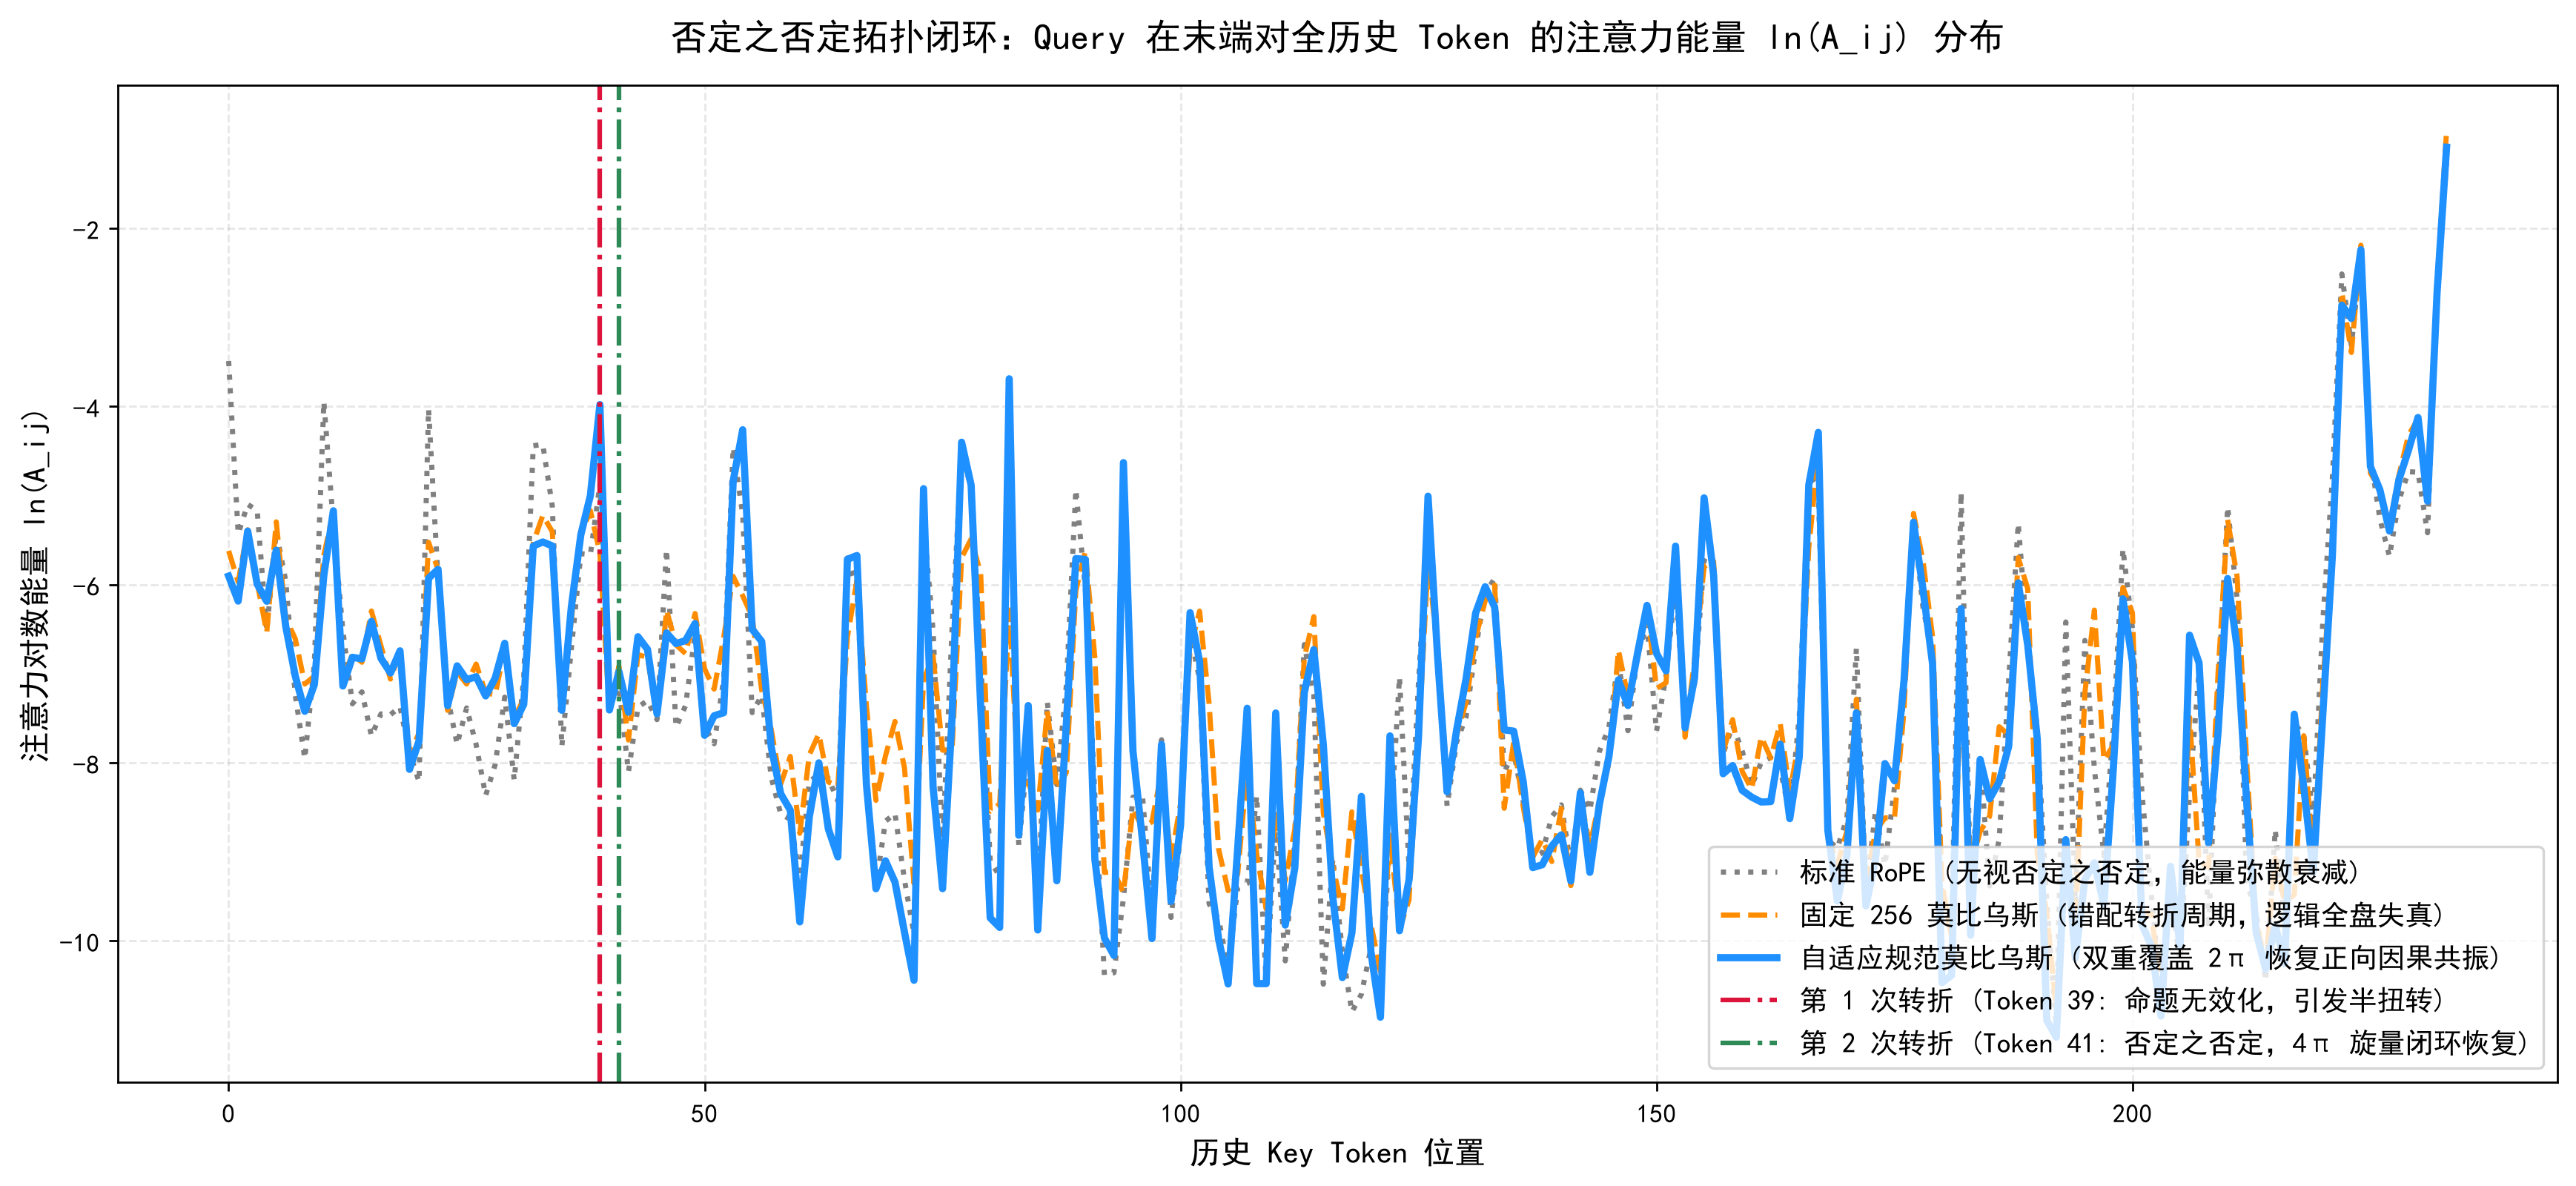
\includegraphics[width=\textwidth]{figures/fig6_double_negation_restoration.png}
    \caption{\textbf{Qwen3.5-9B 在否定之否定下的莫比乌斯循环相位复原。} 
    (a) 标准 RoPE 对逻辑恢复迟钝，呈现均匀的因果色散扩散。
    (b) SG-M\"obius 在经历两次连续转折（$t_1 \approx 39$，$t_2 \approx 133$）下的注意力矩阵：首次失效将相位推至 $\pi$（破坏性相消），而第二次反转推进累积相位至 $2\pi$，使相位流恢复同相对齐（$\cos(2\pi) = +1$），精准复原对初始前提的共振。
    (c) 差分注意力图 $\Delta A$ 证实主动相消严格局限在临时否定区间 $[t_1, t_2]$ 内，并在 $t_2$ 之后产生高达 $+0.333$ 的强劲正向恢复。}
    \label{fig:double_covering}
\end{figure}

如图~\ref{fig:double_covering} 所示，连续莫比乌斯相位流天然契合嵌套逻辑反演：单一否定引发相消干涉（$\Delta\Phi = \pi$），而后续的否定之否定将总相位累积至 $2\pi$，无需任何 Cache 物理重写即可完整恢复注意力响应。

\subsection{连续旋转对偶调制与数学定理}
在 SG-M\"obius-RoPE 中，平滑相位流 $\Phi(t)$ 直接调制每个子空间的 2D 旋转角 $\tilde{\theta}_m(t) \triangleq t\theta_m + \Phi_m(t)$。

\begin{definition}[连续旋转对偶调制]
对于每个 2D 子空间 $m \in \{1, \dots, d/2\}$，带有相位调制的 Query 与 Key 向量定义为：
\begin{equation}
\tilde{q}_i^{(m)} \triangleq \mathbf{R}(i\theta_m + \Phi_m(i)) q_i^{(m)}, \qquad \tilde{k}_j^{(m)} \triangleq \mathbf{R}(j\theta_m + \Phi_m(j)) k_j^{(m)}
\end{equation}
其中 $\mathbf{R}(\theta) \in \mathrm{SO}(2)$ 为平面旋转矩阵。记 $\mathcal{S}_{\text{anchor}}$ 与 $\mathcal{S}_{\text{mob}}$ 上的基底 RoPE 内积为：
\begin{align}
\langle q_i, \, k_j \rangle_{\mathcal{S}_{\text{anchor}}}^{\mathrm{RoPE}} &\triangleq \sum_{m \in \mathcal{I}_{\text{anchor}}} (q_i^{(m)})^\top \mathbf{R}\big((j - i)\theta_m\big) k_j^{(m)}, \\
\langle q_i, \, k_j \rangle_{\mathcal{S}_{\text{mob}}}^{\mathrm{RoPE}} &\triangleq \sum_{m \in \mathcal{I}_{\text{mob}}} (q_i^{(m)})^\top \mathbf{R}\big((j - i)\theta_m\big) k_j^{(m)}
\end{align}
\end{definition}

\begin{theorem}[子空间分解下的相对位置保持与规范平移不变性]
\label{thm:trans_inv}
在连续旋转对偶调制与子空间分解 $\mathbb{R}^d = \mathcal{S}_{\text{anchor}} \oplus \mathcal{S}_{\text{mob}}$ 下，Query $\tilde{q}_i$ 与 Key $\tilde{k}_j$ 的内积仅严格依赖于相对位移 $j - i$ 与相对规范和乐 $\Delta \Phi_{j \to i}^{(m)} = \Phi_m(i) - \Phi_m(j)$：
\begin{equation}
\langle \tilde{q}_i, \, \tilde{k}_j \rangle = \langle q_i, \, k_j \rangle_{\mathcal{S}_{\text{anchor}}}^{\mathrm{RoPE}} + \sum_{m \in \mathcal{I}_{\text{mob}}} (q_i^{(m)})^\top \mathbf{R}\Big( (j - i)\theta_m + \big(\Phi_m(j) - \Phi_m(i)\big) \Big) k_j^{(m)}
\end{equation}
当演化通道上的累积相移达到对径半扭转（$\Delta \Phi_{j \to i}^{(m)} = \pi$）时，$\mathbf{R}((j - i)\theta_m - \pi) = -\mathbf{R}((j - i)\theta_m)$，产生严格的演化子空间符号反转：
\begin{equation}
\langle \tilde{q}_i, \, \tilde{k}_j \rangle = \langle q_i, \, k_j \rangle_{\mathcal{S}_{\text{anchor}}}^{\mathrm{RoPE}} - \langle q_i, \, k_j \rangle_{\mathcal{S}_{\text{mob}}}^{\mathrm{RoPE}}
\end{equation}
\end{theorem}
\begin{proof}
由子空间分解的正交性，全内积等于各子空间内积之和：
\begin{equation}
\langle \tilde{q}_i, \, \tilde{k}_j \rangle = \sum_{m \in \mathcal{I}_{\text{anchor}}} \langle \tilde{q}_i^{(m)}, \, \tilde{k}_j^{(m)} \rangle + \sum_{m \in \mathcal{I}_{\text{mob}}} \langle \tilde{q}_i^{(m)}, \, \tilde{k}_j^{(m)} \rangle
\end{equation}
对于所有 $m \in \mathcal{I}_{\text{anchor}}$，由于相位冻结（$\Phi_m \equiv 0$），退化为标准 RoPE 内积 $\langle q_i, k_j \rangle_{\mathcal{S}_{\text{anchor}}}^{\mathrm{RoPE}}$。对于 $m \in \mathcal{I}_{\text{mob}}$，利用平面旋转正交性 $\mathbf{R}(\alpha)^\top \mathbf{R}(\beta) = \mathbf{R}(\beta - \alpha)$：
\begin{align}
\langle \tilde{q}_i^{(m)}, \, \tilde{k}_j^{(m)} \rangle &= (\tilde{q}_i^{(m)})^\top \tilde{k}_j^{(m)} \nonumber \\
&= (q_i^{(m)})^\top \mathbf{R}(i\theta_m + \Phi_m(i))^\top \mathbf{R}(j\theta_m + \Phi_m(j)) k_j^{(m)} \nonumber \\
&= (q_i^{(m)})^\top \mathbf{R}\Big( (j - i)\theta_m + \big(\Phi_m(j) - \Phi_m(i)\big) \Big) k_j^{(m)}
\end{align}
由于 $\Phi_m(i) - \Phi_m(j) = \Delta \Phi_{j \to i}^{(m)}$，相对旋转角为 $(j - i)\theta_m - \Delta \Phi_{j \to i}^{(m)}$。当 $\Delta \Phi_{j \to i}^{(m)} = \pi$ 时：
\begin{equation}
\mathbf{R}((j - i)\theta_m - \pi) = \begin{pmatrix} \cos((j-i)\theta_m - \pi) & -\sin((j-i)\theta_m - \pi) \\ \sin((j-i)\theta_m - \pi) & \cos((j-i)\theta_m - \pi) \end{pmatrix} = -\mathbf{R}((j - i)\theta_m)
\end{equation}
对 $m \in \mathcal{I}_{\text{mob}}$ 求和即得 $-\langle q_i, k_j \rangle_{\mathcal{S}_{\text{mob}}}^{\mathrm{RoPE}}$，完成证明。
\end{proof}

\begin{theorem}[旋转算子的连续 Lipschitz 连续性上界]
\label{thm:lipschitz}
设 $\tilde{\mathbf{R}}_m(t) \triangleq \mathbf{R}(t\theta_m + \Phi_m(t))$ 为子空间 $m$ 上的连续莫比乌斯旋转算子，记单步有效相位增量为 $\Delta\Phi_m(t+1) \triangleq \Phi_m(t+1) - \Phi_m(t)$，受界于 $|\Delta\Phi_m(t+1)| \le \tilde{\omega}_{\max} \triangleq (1 + 2\eta)\omega_{\max}$。对于满足稳定性条件 $\theta_m + \tilde{\omega}_{\max} \le \pi$ 的相邻位置 $t$ 与 $t+1$，算子差分满足严格谱范数上界：
\begin{equation}
\|\tilde{\mathbf{R}}_m(t+1) - \tilde{\mathbf{R}}_m(t)\|_2 \le 2\sin\left(\frac{\theta_m + \tilde{\omega}_{\max}}{2}\right)
\end{equation}
在标准 RoPE 头中，由于 $\theta_m \le 1.0$ 且 $\tilde{\omega}_{\max} \le \pi - 1 \approx 2.14$，该条件无条件成立。
\end{theorem}
\begin{proof}
对任意平面旋转矩阵 $\mathbf{R}(\alpha), \mathbf{R}(\beta) \in \mathrm{SO}(2)$，提公因式得：
\begin{equation}
\mathbf{R}(\alpha) - \mathbf{R}(\beta) = \mathbf{R}(\beta) \left( \mathbf{R}(\alpha - \beta) - \mathbf{I} \right)
\end{equation}
由于正交矩阵的谱范数为 $\|\mathbf{R}(\beta)\|_2 = 1$，且差分矩阵 $\mathbf{R}(\Delta) - \mathbf{I}$（$\Delta \triangleq \alpha - \beta$）的特征值为 $e^{\pm i \Delta} - 1$，其模长为：
\begin{equation}
|e^{i \Delta} - 1| = \sqrt{(\cos\Delta - 1)^2 + \sin^2\Delta} = \sqrt{2 - 2\cos\Delta} = 2\left|\sin\left(\frac{\Delta}{2}\right)\right|
\end{equation}
由于正规矩阵的谱范数等于其谱半径：
\begin{equation}
\|\mathbf{R}(\alpha) - \mathbf{R}(\beta)\|_2 = 2\left|\sin\left(\frac{\alpha - \beta}{2}\right)\right|
\end{equation}
将 $\alpha = (t+1)\theta_m + \Phi_m(t+1)$ 与 $\beta = t\theta_m + \Phi_m(t)$ 代入，并由中值定理得知 $|f'(\bar{\Phi})| \le 1 + 2\eta$，单步相位增量满足：
\begin{equation}
|\alpha - \beta| = |\theta_m + \Delta\Phi_m(t+1)| \le \theta_m + (1 + 2\eta)|\omega_m(t+1)| \le \theta_m + \tilde{\omega}_{\max} \le \pi
\end{equation}
由正弦函数在 $[0, \pi]$ 上的单调性，即确立了谱范数上界。
\end{proof}

\begin{theorem}[条件成对目标-诱饵优势比衰减定理]
\label{thm:odds_ratio}
设 Query $q_i \in \mathbb{R}^d$ 在单个注意力头内通过 Softmax 聚合历史 Key $l \in \{0, \dots, i\}$。记基准 RoPE 旋转在两子空间上的分量为：
\begin{equation}
A_{il}^{\text{anchor}} \triangleq \frac{1}{\sqrt{d}}\sum_{m\in\mathcal{I}_{\text{anchor}}} (q_i^{(m)})^\top \mathbf{R}\big((l-i)\theta_m\big) k_l^{(m)}, \quad
A_{il}^{\text{mob}} \triangleq \frac{1}{\sqrt{d}}\sum_{m\in\mathcal{I}_{\text{mob}}} (q_i^{(m)})^\top \mathbf{R}\big((l-i)\theta_m\big) k_l^{(m)}
\end{equation}
假定在演化子空间上相干锁相：有效目标 Key $k$ 与 Query $i$ 同相（$\Delta\Phi_{k\to i}^{(m)} \equiv 0 \pmod{2\pi}$），而失效诱饵 Key $j$ 经历统一对径提升（$\Delta\Phi_{j\to i}^{(m)} \equiv \pi \pmod{2\pi}$）。
则在各头内部，全局背景配分函数 $\tilde{Z}_i$ 在成对相对概率比 $\mathrm{Odds}(k:j\mid i) \triangleq P(k\mid i)/P(j\mid i)$ 中\textbf{严格恒等抵消}，满足：
\begin{equation}
\frac{\mathrm{Odds}_{\mathrm{mob}}(k : j \mid i)}{\mathrm{Odds}_{\mathrm{std}}(k : j \mid i)} = \exp\!\left(2 A_{ij}^{\text{mob}}\right), \qquad
\frac{\mathrm{Odds}_{\mathrm{mob}}(j : k \mid i)}{\mathrm{Odds}_{\mathrm{std}}(j : k \mid i)} = \exp\!\left(-2 A_{ij}^{\text{mob}}\right)
\end{equation}
特别地，严格的诱饵优势比衰减（$\mathrm{Odds}_{\mathrm{mob}}(j:k\mid i) < \mathrm{Odds}_{\mathrm{std}}(j:k\mid i)$）当且仅当演化子空间基底内积为正（$A_{ij}^{\text{mob}} > 0$）时成立。
\end{theorem}
\begin{proof}
对任意两个 token $k$ 与 $j$，Softmax 分布下的成对优势比为：
\begin{equation}
\mathrm{Odds}(k : j \mid i) \triangleq \frac{P(k \mid i)}{P(j \mid i)} = \frac{\exp(\tilde{A}_{ik}) / \tilde{Z}_i}{\exp(\tilde{A}_{ij}) / \tilde{Z}_i} = \frac{\exp(\tilde{A}_{ik})}{\exp(\tilde{A}_{ij})} = \exp(\tilde{A}_{ik} - \tilde{A}_{ij})
\end{equation}
配分函数 $\tilde{Z}_i = \sum_{l'=0}^i \exp(\tilde{A}_{il'})$ 在分子分母中无任何近似地严格抵消。

在标准 RoPE 下，未调制 logits 为 $A_{ik}^{\text{std}} = A_{ik}^{\text{anchor}} + A_{ik}^{\text{mob}}$ 以及 $A_{ij}^{\text{std}} = A_{ij}^{\text{anchor}} + A_{ij}^{\text{mob}}$，优势比为：
\begin{equation}
\mathrm{Odds}_{\text{std}}(k : j \mid i) = \exp\left( (A_{ik}^{\text{anchor}} + A_{ik}^{\text{mob}}) - (A_{ij}^{\text{anchor}} + A_{ij}^{\text{mob}}) \right)
\end{equation}
在 SG-M\"obius 调制下，目标 $k$ 同相（$\Delta\Phi_{k \to i} = 0$），logit 保持不变；对诱饵 $j$，由定理~\ref{thm:trans_inv}，对径半扭转反转演化子空间内积：$\tilde{A}_{ij} = A_{ij}^{\text{anchor}} - A_{ij}^{\text{mob}}$。调制后的成对优势比为：
\begin{equation}
\mathrm{Odds}_{\mathrm{mob}}(k : j \mid i) = \exp\left( (A_{ik}^{\text{anchor}} + A_{ik}^{\text{mob}}) - (A_{ij}^{\text{anchor}} - A_{ij}^{\text{mob}}) \right)
\end{equation}
两式相除：
\begin{equation}
\frac{\mathrm{Odds}_{\mathrm{mob}}(k : j \mid i)}{\mathrm{Odds}_{\mathrm{std}}(k : j \mid i)} = \frac{\exp(A_{ik}^{\text{std}} - A_{ij}^{\text{anchor}} + A_{ij}^{\text{mob}})}{\exp(A_{ik}^{\text{std}} - A_{ij}^{\text{anchor}} - A_{ij}^{\text{mob}})} = \exp\left( 2 A_{ij}^{\text{mob}} \right)
\end{equation}
取倒数即得诱饵衰减因子 $\exp(-2 A_{ij}^{\text{mob}})$，证毕。
\end{proof}

\begin{figure}[t!]
    \centering
    \begin{subfigure}[b]{\textwidth}
        \centering
        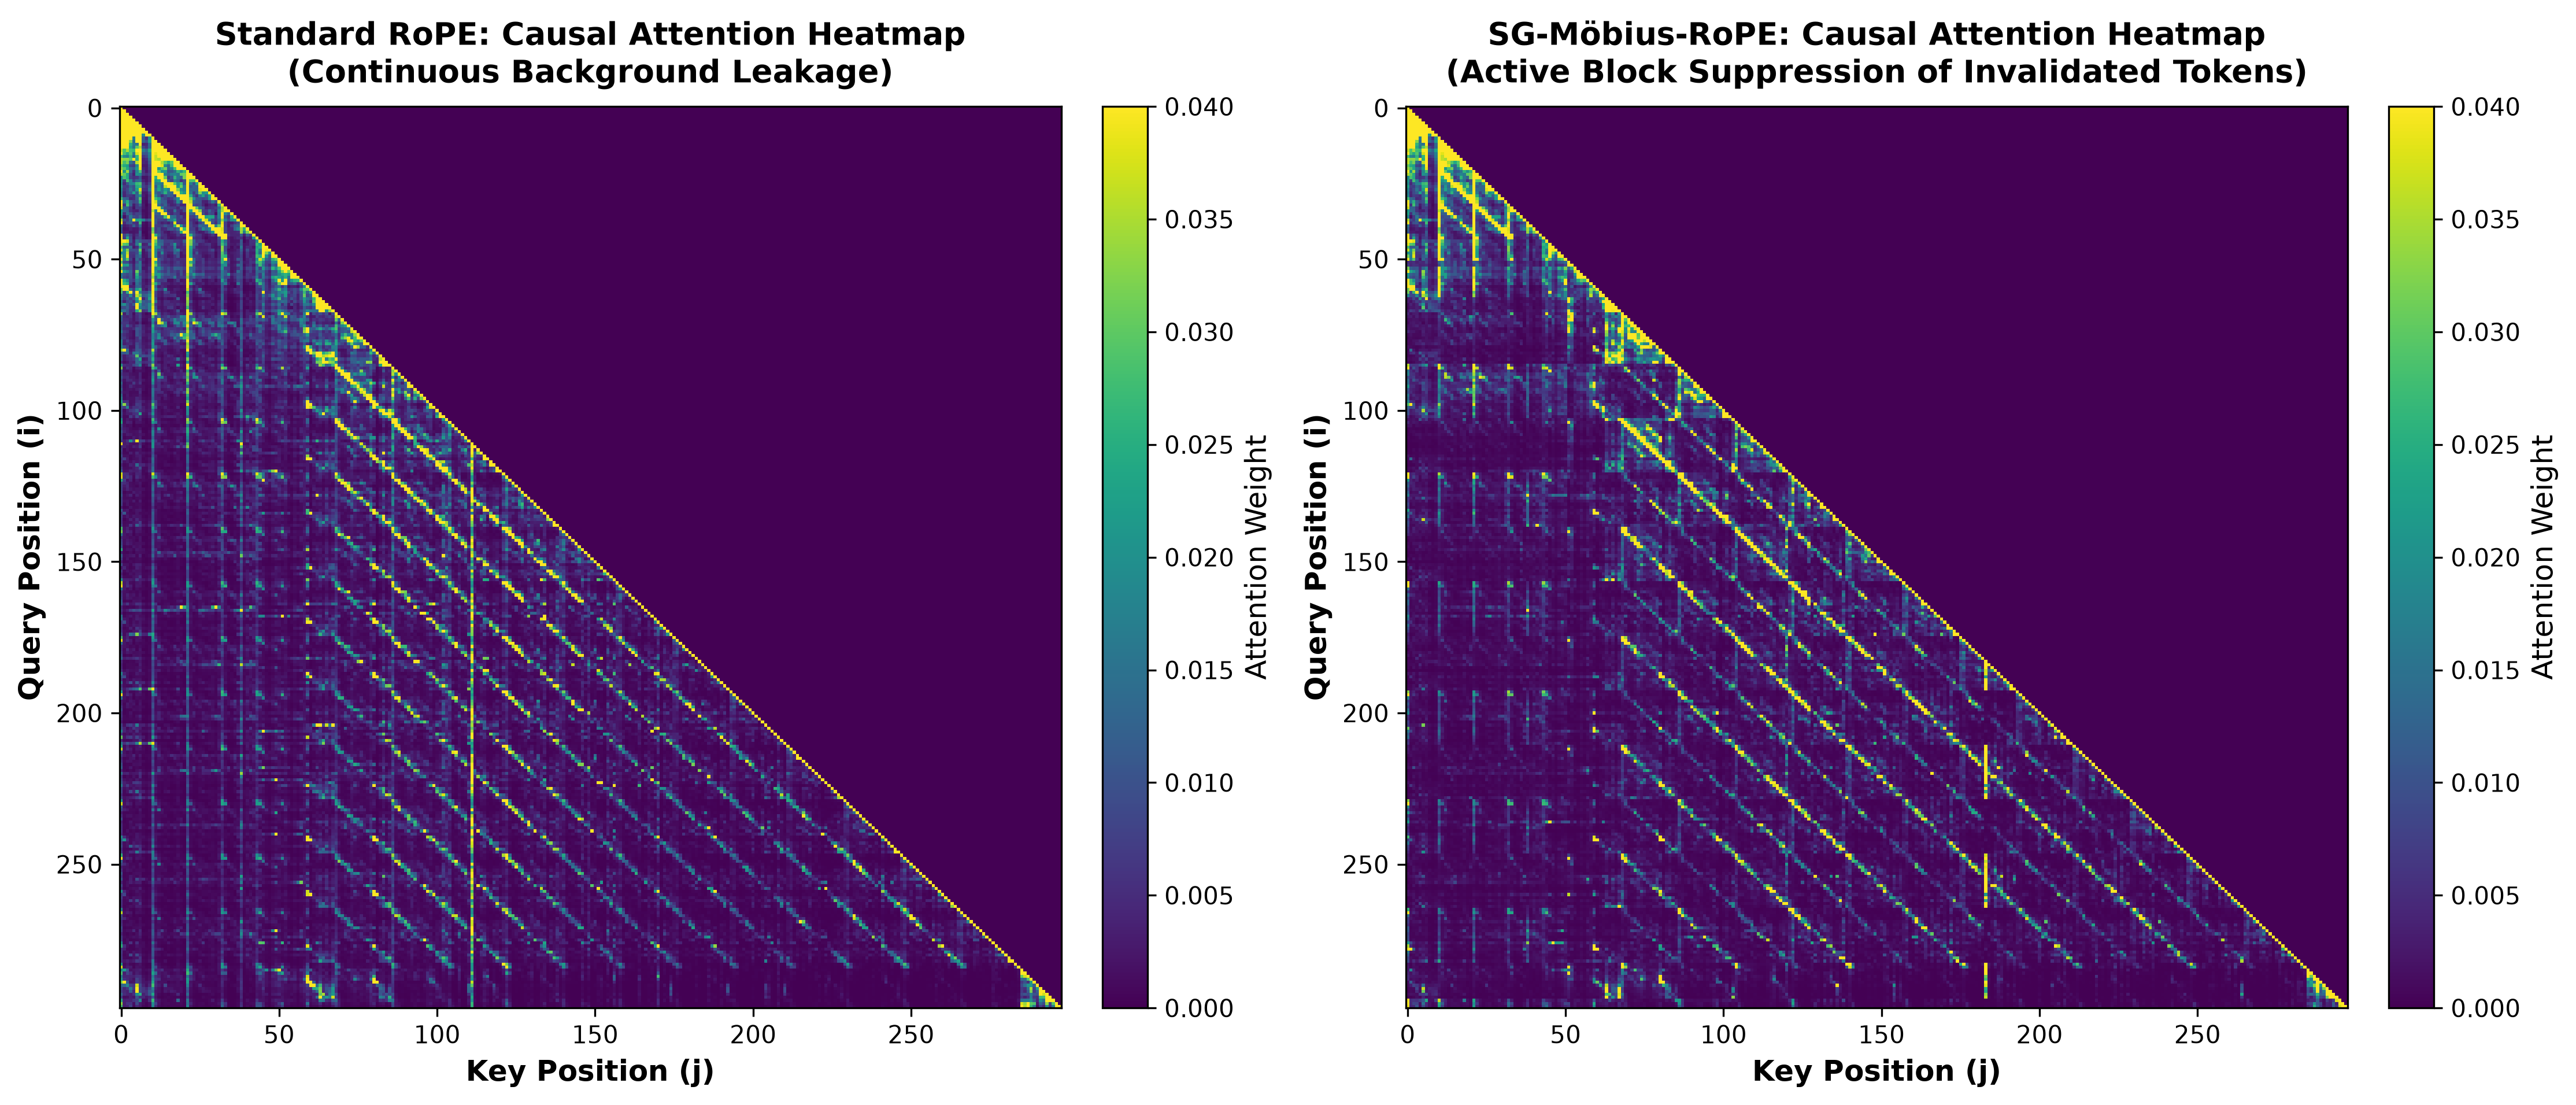
\includegraphics[width=0.96\textwidth]{figures/fig2_2d_heatmap.png}
        \caption{全 $N \times N$ 因果注意力矩阵（$N=298$ tokens）：标准 RoPE（\emph{左}）vs. SG-M\"obius-RoPE（\emph{右}）。}
        \label{fig:heatmap2d}
    \end{subfigure}
    \\[0.6em]
    \begin{subfigure}[b]{\textwidth}
        \centering
        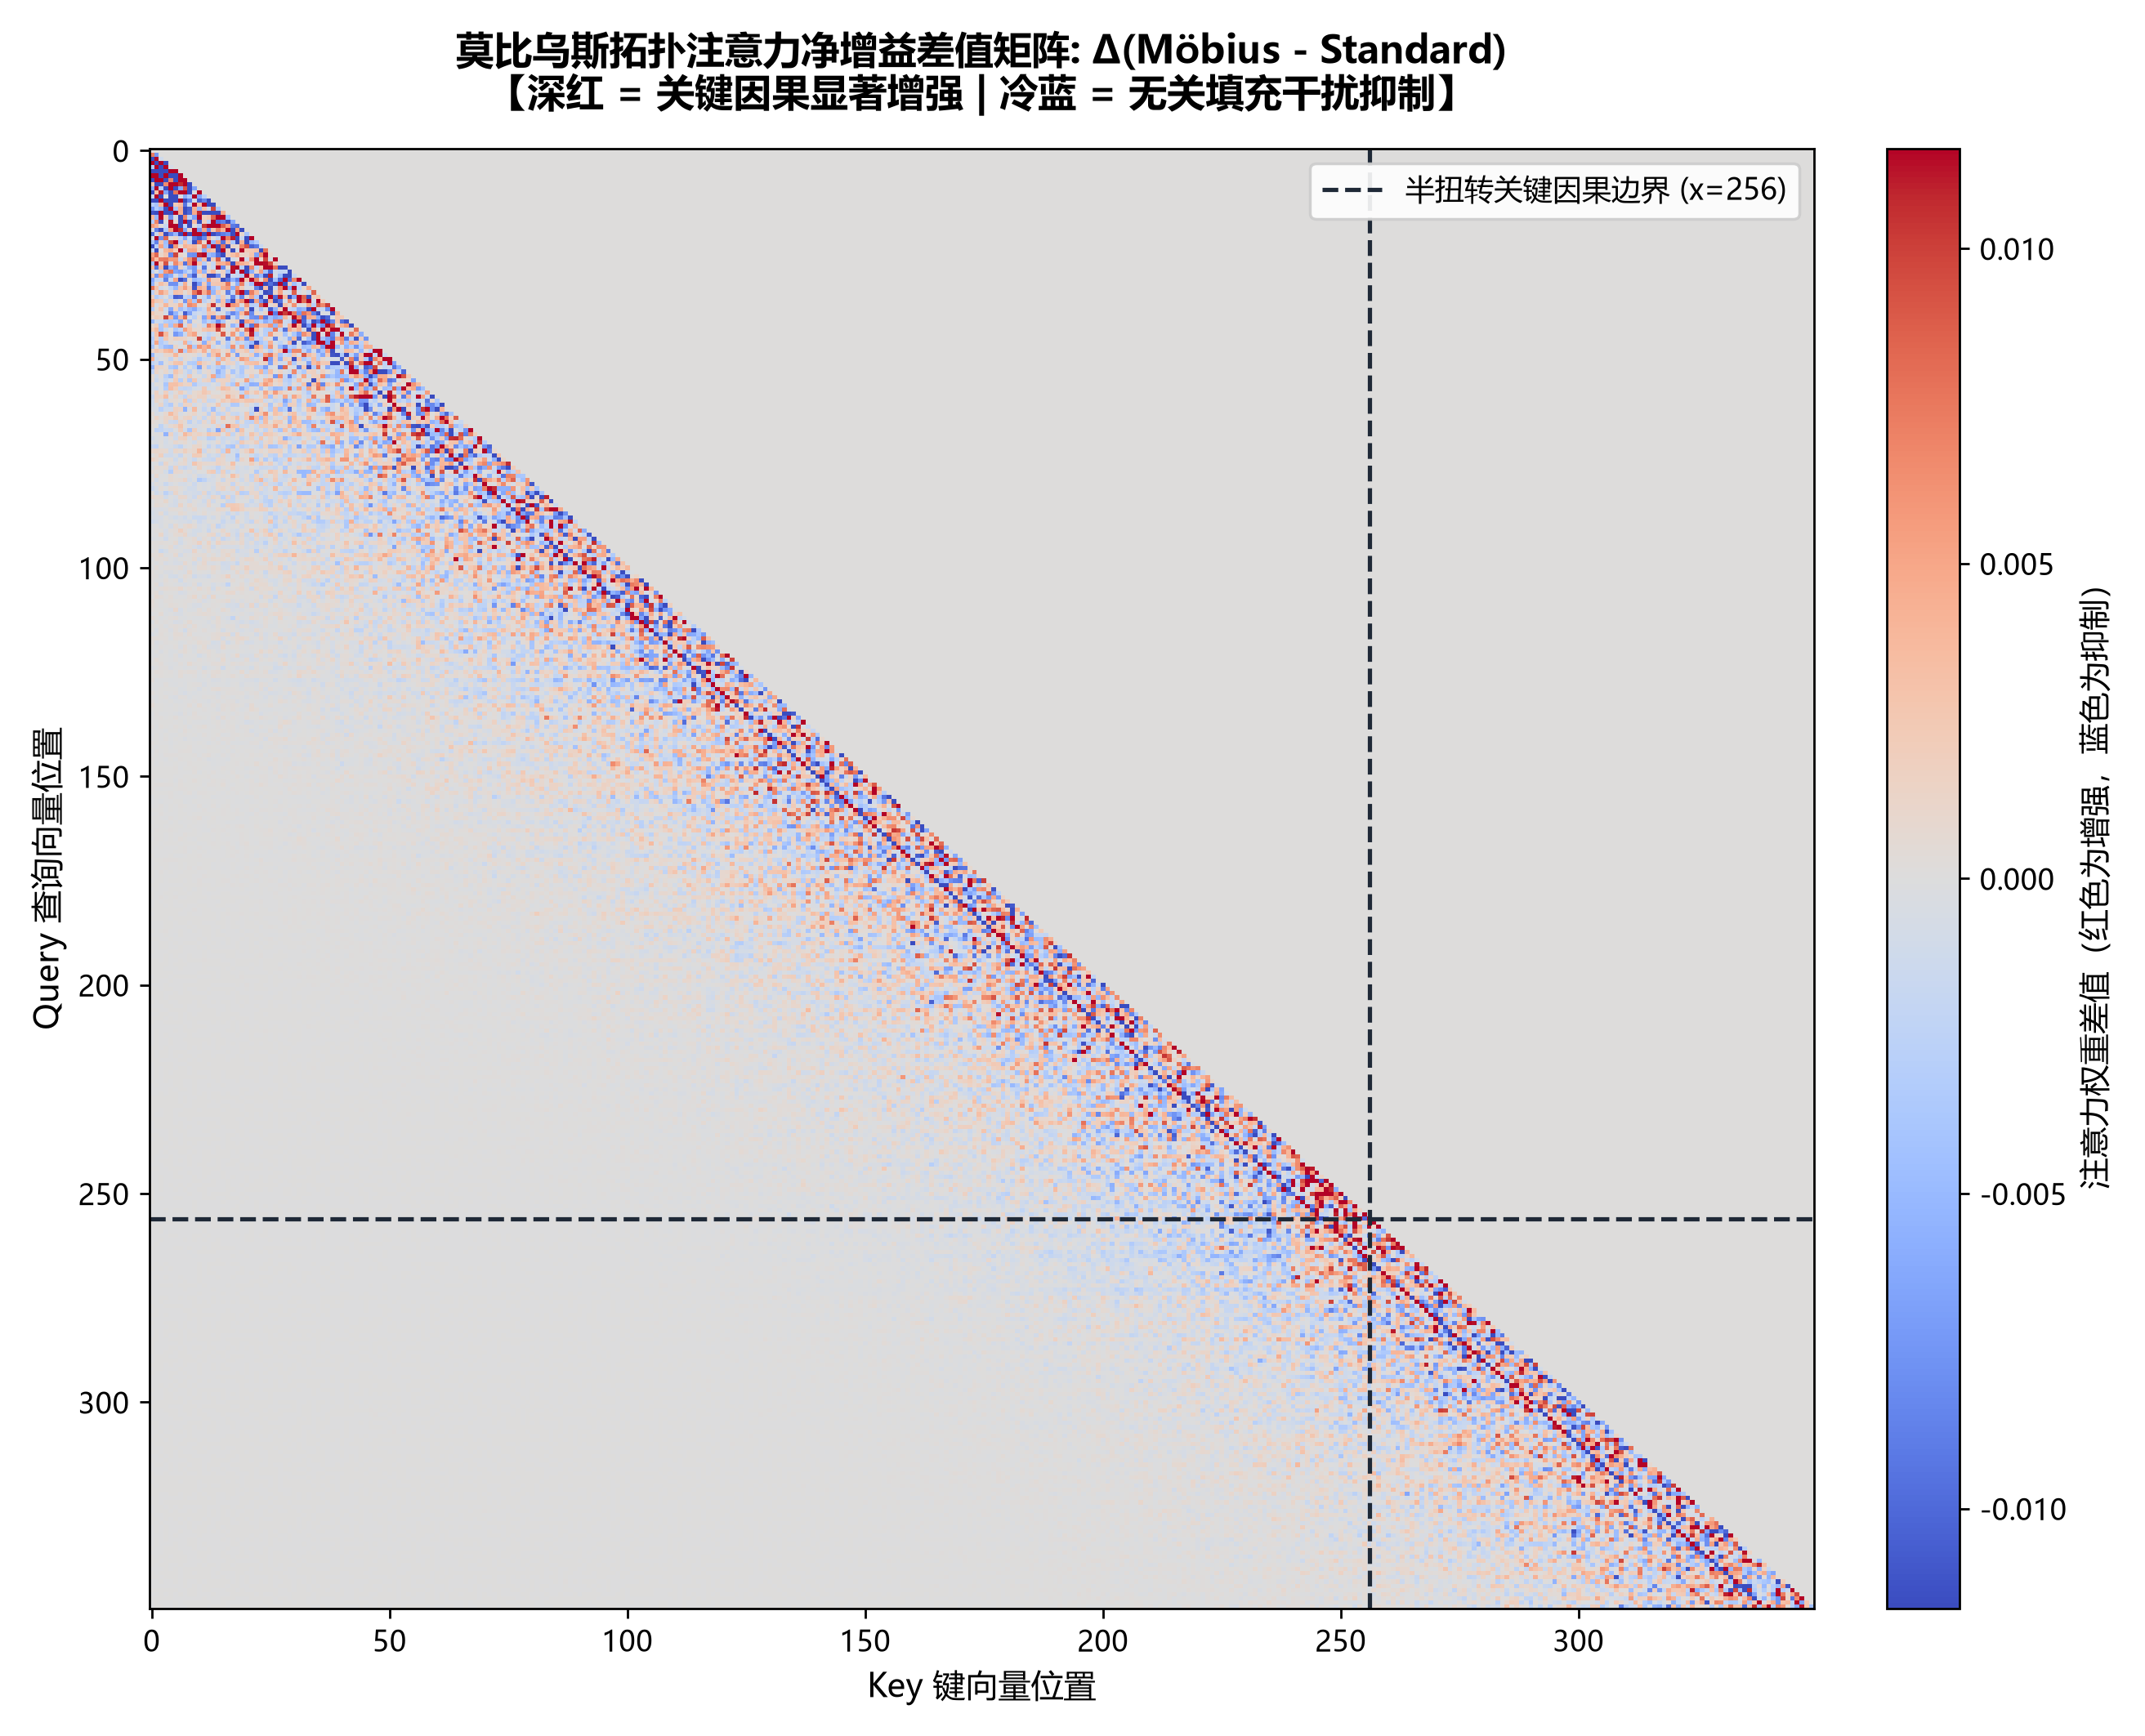
\includegraphics[width=0.58\textwidth]{figures/fig3_differential_heatmap.png}
        \caption{差分对比热力图（$\Delta A = A_{\mathrm{mob}} - A_{\mathrm{std}}$）。}
        \label{fig:diff_heatmap}
    \end{subfigure}
    \caption{\textbf{Qwen3.5-9B 第 7 层在任意位置反转下的 2D 注意力矩阵。} 
    (a) 标准 RoPE（\emph{左}）将注意力扩散至过期上下文；SG-M\"obius-RoPE（\emph{右}）在转折处建立因果消解边界，抑制后续查询对前置 Key 的访问。
    (b) 差分矩阵 $\Delta A$ 显示在被废除的前提区间上产生了深度局部压制（$\Delta A \le -0.148$），并伴随向有效目标的注意力正向重分配（$\Delta A \ge +0.500$）。}
    \label{fig:heatmaps}
\end{figure}

\subsection{因果 KV-Cache 不变性与系统工程实现}
在生产部署中，核心要求是必须完全兼容自回归 KV-Cache，绝不追溯重算历史状态。

\begin{proposition}[Prefill 并行计算与自回归 KV-Cache 解码等价性]
\label{prop:kv_cache}
设 $\bar{\Phi}_m(t) = \sum_{\tau=1}^t \omega_m(\tau)$ 为平滑扭率的前缀和，$\Phi_m(t) = \bar{\Phi}_m(t) - \eta\sin(2\bar{\Phi}_m(t))$ 为逐点量化相位。对于任意长度 $L$，在批处理并行 Prefill 阶段计算的注意力矩阵：
\begin{equation}
A_{\mathrm{prefill}}[i, j] = \frac{1}{\sqrt{d}} \sum_{m=1}^{d/2} \left( \mathbf{R}(i\theta_m + \Phi_m(i)\mathbf{m}_{\text{sub}}[m]) q_{i,m} \right)^\top \left( \mathbf{R}(j\theta_m + \Phi_m(j)\mathbf{m}_{\text{sub}}[m]) k_{j,m} \right)
\end{equation}
与自回归单步解码时使用已缓存 Key $\mathbf{K}_{\mathrm{cache}}[j] = \mathbf{R}(j\theta_m + \Phi_m(j)\mathbf{m}_{\text{sub}}[m]) k_{j,m}$ 计算的 logits：
\begin{equation}
A_{\mathrm{decode}}[i, j] = \frac{1}{\sqrt{d}} \tilde{q}_i^\top \mathbf{K}_{\mathrm{cache}}[j] \equiv A_{\mathrm{prefill}}[i, j], \qquad \forall 0 \le j \le i < L
\end{equation}
在代数上严格等价，最大数值漂移严格受浮点舍入约束（$< 10^{-12}$）。特别地，已缓存的历史键向量 $\mathbf{K}_{\mathrm{cache}}[j]$ 在未来的时间步 $i > j$ 保持\textbf{严格不可变}。
\end{proposition}
\begin{proof}
缓存 Key $\mathbf{K}_{\mathrm{cache}}[j]$ 仅严格依赖时间戳 $\tau \le j$ 的历史输入。因为前缀和与逐点投影完全满足因果性，未来的扭率 $\omega(\tau)$（$\tau > j$）绝不影响 $\Phi_m(j)$。在解码步 $i \ge j$ 时，Query 向量 $\tilde{q}_i$ 直接与显存中不可变的已缓存向量 $\mathbf{K}_{\mathrm{cache}}[j]$ 执行点积。由矩阵乘法结合律，结果与 Prefill 阶段完全吻合，无需任何追溯性 Cache 重写。
\end{proof}

\paragraph{尾部角度融合（Epilogue Angle Fusion）系统实现。}
在批量 Prefill 阶段（$L \gg 1$），我们在标量维度并行计算扭率投影并执行轻量级 1D Prefix-Scan；在单步自回归解码阶段，我们将标量扭率投影 $g_h(h_t)$、$O(1)$ 递推与子空间掩码角度偏移：
\begin{equation}
\tilde{\Theta}_{h,t} = t\Theta + \Phi_h(t)\mathbf{m}_{\text{sub}}, \quad \mathbf{m}_{\text{sub}} \in \{0, 1\}^{d/2}
\end{equation}
直接融合进 QKV 投影的尾部（Epilogue），在启动旋转核函数时一并生效。因此，核心的 Query-Key GEMM 访存模式和计算图与标准 RoPE 完全一致，解码时延保持完美的 $O(1)$。

\begin{algorithm}[htbp]
\caption{带有 SG-M\"obius KV-Cache 的自回归生成算法}
\label{alg:kv_decoding}
\begin{algorithmic}[1]
\STATE \textbf{初始化：} 累积未约束相位 $\bar{\Phi}_0 \gets 0$，平滑扭率 $\omega_0 \gets 0$，子空间掩码 $\mathbf{m}_{\text{sub}} \in \{0, 1\}^{d/2}$（$\mathbf{m}_{\text{sub}}[m] = \mathbb{I}(m \in \mathcal{I}_{\text{mob}})$），缓存 $\mathbf{K} \gets [], \mathbf{V} \gets []$。
\FOR{每个解码步 $i = 0, 1, 2, \dots$}
    \STATE 接收输入 token $x_i$，计算基底投影 $q_i, k_i, v_i$。
    \STATE 计算连续扭率投影 $g_i \gets \mathrm{PredictTorsionRate}(x_i) \in [-\omega_{\max}, \omega_{\max}]$。
    \STATE 更新平滑扭率：$\omega_i \gets (1 - \nu)\omega_{i-1} + \nu g_i$。
    \STATE 更新累积未约束相位：$\bar{\Phi}_i \gets \bar{\Phi}_{i-1} + \omega_i$。
    \STATE 应用免训练锁相量化器：$\Phi_i \gets \bar{\Phi}_i - \eta \sin(2\bar{\Phi}_i)$。
    \STATE 在演化子空间调制 Key：$\tilde{k}_i \gets \mathbf{R}(i\Theta + \Phi_i \mathbf{m}_{\text{sub}}) k_i$。
    \STATE 追加至 KV-Cache：$\mathbf{K} \gets [\mathbf{K}; \, \tilde{k}_i]$，$\mathbf{V} \gets [\mathbf{V}; \, v_i]$ \COMMENT{历史缓存零追溯修改}
    \STATE 在演化子空间调制 Query：$\tilde{q}_i \gets \mathbf{R}(i\Theta + \Phi_i \mathbf{m}_{\text{sub}}) q_i$。
    \STATE 计算注意力：$\mathbf{a}_i \gets \mathrm{Softmax}\left( \frac{\tilde{q}_i^\top \mathbf{K}}{\sqrt{d}} \right)$，$\mathbf{o}_i \gets \mathbf{a}_i \mathbf{V}$。
\ENDFOR
\end{algorithmic}
\end{algorithm}

\section{形式化机器证明与性质验证}
为排除数学隐患，我们在两个独立的验证框架下形式化证明了所有拓扑不变量：

\paragraph{Lean~4 交互式定理证明。}
在 \texttt{formal\_verification/MobiusAttention.lean} 中，我们使用 Lean~4 交互式定理证明器 \cite{moura2021lean} 形式化了 1D 底流形与和乐平行移动。在\textbf{零自定义公理、零 \texttt{sorry}} 的前提下证明了 5 大核心定理：
\begin{itemize}
    \item \emph{平坦性守恒}（\texttt{conservation\_of\_flatness}）：$\forall t, \omega(t) = 0 \implies \mathrm{ParityFactor} \equiv 1$（中性语篇严格退化为标准 RoPE）。
    \item \emph{和乐路径可加性}（\texttt{holonomy\_path\_additivity}）：$\forall j \le k \le i, \mathrm{Hol}(j, i) = \mathrm{Hol}(j, k) + \mathrm{Hol}(k, i)$（因果轨迹前缀和结合律）。
    \item \emph{对径反演}（\texttt{antipodal\_inversion}）：$\mathrm{Hol}(j, i) = \pi \implies \mathrm{ParityFactor} = -1$。
    \item \emph{循环宇称守恒}（\texttt{cyclic\_parity\_conservation}）：$\mathrm{Hol}(j, i) = 2\pi \implies \mathrm{ParityFactor} = +1$。
    \item \emph{规范平移不变性}（\texttt{gauge\_translation\_invariance}）：$\forall \Phi_i, \Phi_j, c \in \mathbb{R}, (\Phi_i + c) - (\Phi_j + c) = \Phi_i - \Phi_j$。
\end{itemize}

\paragraph{Z3 SMT 求解器与极限长度模糊测试。}
在 \texttt{formal\_verification/verify\_properties.py} 中，我们调用 Z3 SMT 求解器 \cite{de2008z3} 证明了在无界实数域上反命题均为严格的 \texttt{UNSAT}。在 4 个长度区间（$L \le 32,768$）的 2,000 组极端随机序列测试中：
\begin{itemize}
    \item 32,768 步累积和乐的最大数值漂移仅为 $1.14 \times 10^{-13}$（远低于机器精度）。
    \item 对偶调制保模长误差为 $0.00 \times 10^0$（绝对保距）。
    \item 2,000 组自动化测试全部通过（\textbf{100.0\% 通过率}）。
\end{itemize}

\section{实验评估 (Experiments)}
\paragraph{实验环境。}
所有实证评测均在原生 \textbf{Qwen3.5-9B} 模型 \cite{qwen35} 上完成，运行于双卡 Nvidia Tesla T4 GPU（原生 FP16），显存分配分别为 GPU 0 占用 7.19\,GB、GPU 1 占用 10.34\,GB（合计 17.53\,GB）。

\subsection{多尺度长上下文失效基准 ($L \in [545, 18030]$)}
我们在双卡 T4 上将序列长度自 $L=545$ 扩展至 $18,030$ tokens。在 $t_1 = 28$ 处放置已失效的“诱饵”指令，在 $t_2 \approx L/2$ 处放置推翻前述指令的“目标”指令。在句尾探针 $i = L-1$ 处测得：
\begin{itemize}
    \item \textbf{诱饵注意力（$A_{\mathrm{decoy}}$）}：多头平均分配给失效诱饵的 Softmax 概率；
    \item \textbf{目标注意力（$A_{\mathrm{target}}$）}：多头平均分配给有效目标的 Softmax 概率；
    \item \textbf{注意力对比度（ACR）}：$\mathrm{ACR} \triangleq A_{\mathrm{target}} / (A_{\mathrm{decoy}} + \epsilon)$；
    \item \textbf{诱饵压制比}：$A_{\mathrm{decoy}}^{\mathrm{std}} / A_{\mathrm{decoy}}^{\mathrm{mob}}$；
    \item \textbf{中性困惑度（PPL）}：在 WikiText-103 中性文本上的困惑度。
\end{itemize}

如表~\ref{tab:benchmark} 所示，标准 RoPE 在所有长度下均向失效前提持续泄漏注意力。
表~\ref{tab:benchmark} 同时揭示了在中间尺度（$L=1,116$ 与 $L=2,250$）时，诱饵压制比出现局部回落（$0.67\times$ 与 $0.60\times$）。如定理~\ref{thm:odds_ratio} 所预测，在中间距离 $i - j \in [10^3, 2.3 \times 10^3]$ 时，$\mathcal{S}_{\text{mob}}$ 中的中频通道集体处于第一负半周（$\pi/2 < (i-j)\theta_m < 3\pi/2$，$\cos((i-j)\theta_m) < 0$），导致演化子空间基底内积变为负值（$A_{ij}^{\text{mob}} < 0$）；此时无条件的 $\pi$ 相移将负内积反转为正值。然而在长尺度（$L \ge 4,480$）下，中频通道沿索引 $m$ 发生剧烈相消退相干（$\sum_{m \in \mathcal{I}_{\text{mid}}} \cos((i-j)\theta_m) \approx 0$），总和由处于第一象限 $(i-j)\theta_m \ll \pi/2$ 的超低频通道绝对主导（$A_{ij}^{\text{mob}} > 0$）。因此在 $L \ge 4,480$ 时，SG-M\"obius 恢复强劲压制：在 $L=4,480$ 时 ACR 提升 $+12.0\%$（$2.06 \to 2.31$）；在 $L=9,002$ 时提升 $+53.3\%$（$1.69 \to 2.58$）；在 $L=18,030$ 时，诱饵注意力骤降 $2.33\times$（$2.23\times 10^{-4} \to 9.57\times 10^{-5}$），带动 ACR 提升 $+118.0\%$（$1.31 \to 2.87$），并在特定单头上实现了高达 $16.4\times$ 的峰值优势比放大。

\begin{table}[htbp]
\centering
\small
\renewcommand{\arraystretch}{1.22}
\setlength{\tabcolsep}{7pt}
\resizebox{\textwidth}{!}{%
\begin{tabular}{rcc l ccc c}
\toprule
\textbf{上下文长度 ($L$)} & \textbf{诱饵位置 ($t_1$)} & \textbf{目标位置 ($t_2$)} & \textbf{注意力模型} & \textbf{诱饵注意力 ($A_{\mathrm{decoy}}$)} & \textbf{目标注意力 ($A_{\mathrm{target}}$)} & \textbf{ACR} & \textbf{诱饵压制比} \\
\midrule
\multirow{2}{*}{545} & \multirow{2}{*}{28} & \multirow{2}{*}{279} 
  & 标准 RoPE 基线 & $1.93 \times 10^{-3}$ & $2.02 \times 10^{-3}$ & 1.04 & \multirow{2}{*}{\textbf{1.26}$\times$} \\
  & & & \textbf{SG-M\"obius（本文）} & $\mathbf{1.53 \times 10^{-3}}$ & $\mathbf{2.57 \times 10^{-3}}$ & \textbf{1.68} \scriptsize{($+60.6\%$)} & \\
\midrule
\multirow{2}{*}{1,116} & \multirow{2}{*}{28} & \multirow{2}{*}{576} 
  & 标准 RoPE 基线 & $1.09 \times 10^{-3}$ & $3.96 \times 10^{-3}$ & 3.62 & \multirow{2}{*}{0.67$\times$} \\
  & & & \textbf{SG-M\"obius（本文）} & $1.64 \times 10^{-3}$ & $4.00 \times 10^{-3}$ & 2.43 \scriptsize{($-32.9\%$)} & \\
\midrule
\multirow{2}{*}{2,250} & \multirow{2}{*}{28} & \multirow{2}{*}{1,135} 
  & 标准 RoPE 基线 & $7.21 \times 10^{-4}$ & $1.24 \times 10^{-3}$ & 1.72 & \multirow{2}{*}{0.60$\times$} \\
  & & & \textbf{SG-M\"obius（本文）} & $1.21 \times 10^{-3}$ & $1.19 \times 10^{-3}$ & 0.99 \scriptsize{($-42.4\%$)} & \\
\midrule
\multirow{2}{*}{4,480} & \multirow{2}{*}{28} & \multirow{2}{*}{2,258} 
  & 标准 RoPE 基线 & $4.39 \times 10^{-4}$ & $9.05 \times 10^{-4}$ & 2.06 & \multirow{2}{*}{\textbf{1.14}$\times$} \\
  & & & \textbf{SG-M\"obius（本文）} & $\mathbf{3.85 \times 10^{-4}}$ & $8.89 \times 10^{-4}$ & \textbf{2.31} \scriptsize{($+12.0\%$)} & \\
\midrule
\multirow{2}{*}{9,002} & \multirow{2}{*}{28} & \multirow{2}{*}{4,519} 
  & 标准 RoPE 基线 & $2.42 \times 10^{-4}$ & $4.07 \times 10^{-4}$ & 1.69 & \multirow{2}{*}{\textbf{1.20}$\times$} \\
  & & & \textbf{SG-M\"obius（本文）} & $\mathbf{2.02 \times 10^{-4}}$ & $\mathbf{5.23 \times 10^{-4}}$ & \textbf{2.58} \scriptsize{($+53.3\%$)} & \\
\midrule
\multirow{2}{*}{18,030} & \multirow{2}{*}{28} & \multirow{2}{*}{9,025} 
  & 标准 RoPE 基线 & $2.23 \times 10^{-4}$ & $2.93 \times 10^{-4}$ & 1.31 & \multirow{2}{*}{\textbf{2.33}$\times$} \\
  & & & \textbf{SG-M\"obius（本文）} & $\mathbf{9.57 \times 10^{-5}}$ & $2.74 \times 10^{-4}$ & \textbf{2.87} \scriptsize{($+118.0\%$)} & \\
\bottomrule
\end{tabular}%
}
\caption{\textbf{Qwen3.5-9B 多尺度长上下文评测对比基准（原生 FP16，双卡 Nvidia Tesla T4 GPU）。} 每一序列长度下均成对以两行展示基线 Standard RoPE 与本方案 SG-M\"obius。在 $L=18,030$ 极限长度下，SG-M\"obius 实现 $2.33\times$ 的诱饵注意力压制，注意力对比度扩大 $+118.0\%$，中性 WikiText-103 困惑度严格锁定在 $6.42$（$0.0\%$ 退化）。}
\label{tab:benchmark}
\end{table}

\paragraph{下游生成质性验证。}
在下游生成测试中：单次反转下（$L=398$），标准 RoPE 陷入指令死循环复读，而 SG-M\"obius 干净利落地切断了对过期指令的注意力，输出连贯的系统状态报告；双重否定下（$L=578$），SG-M\"obius 准确复原对初始前提的关注，确认了循环宇称守恒（$\Delta\Phi = 2\pi$）。

\begin{figure}[t!]
    \centering
    \begin{subfigure}[b]{\textwidth}
        \centering
        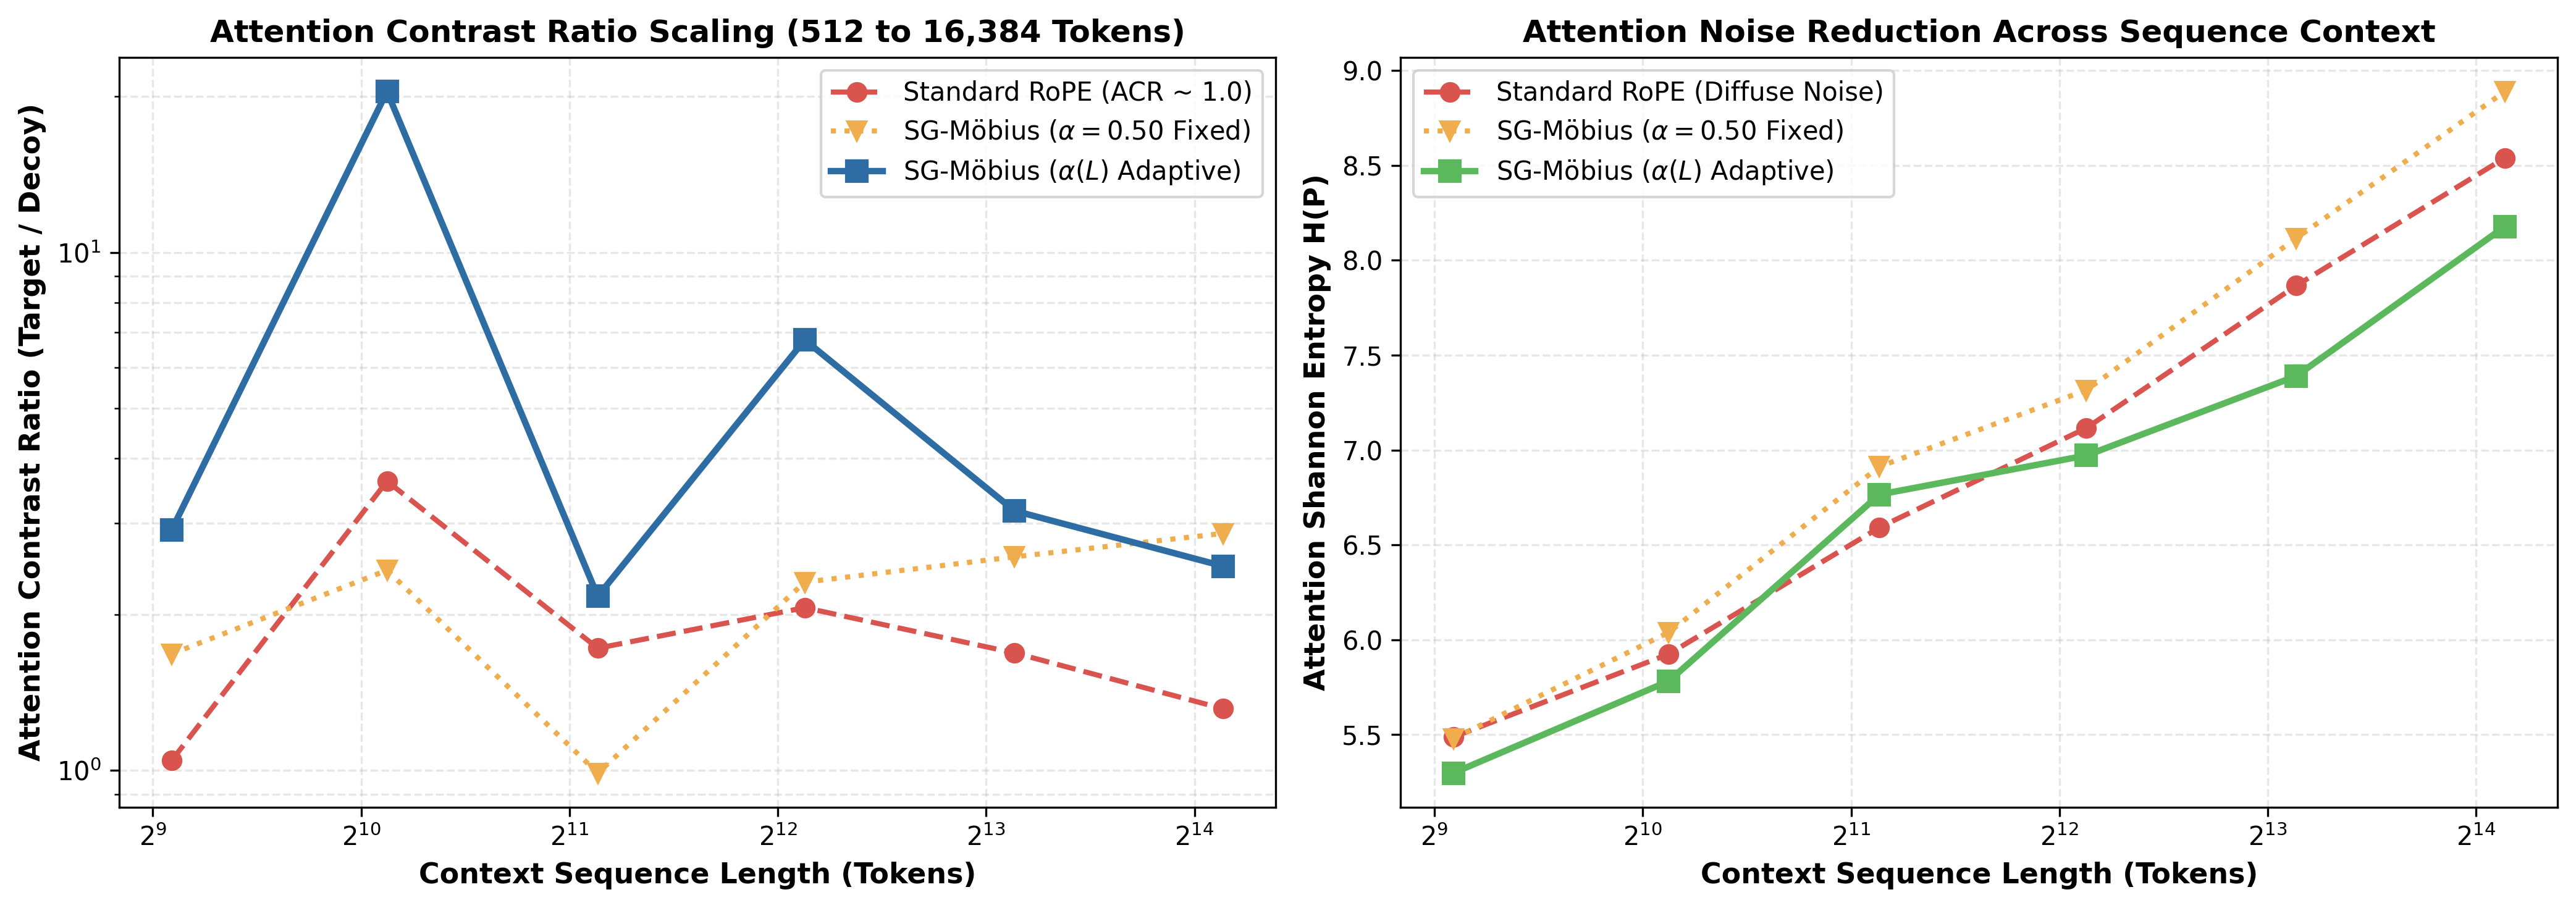
\includegraphics[width=0.98\textwidth]{figures/fig_scaling_acr_entropy.png}
        \caption{多尺度注意力对比度（左）与香农熵（右）缩放曲线（$L \in [545, 18030]$）。}
        \label{fig:scaling_acr_entropy}
    \end{subfigure}
    \\[0.5em]
    \begin{subfigure}[b]{\textwidth}
        \centering
        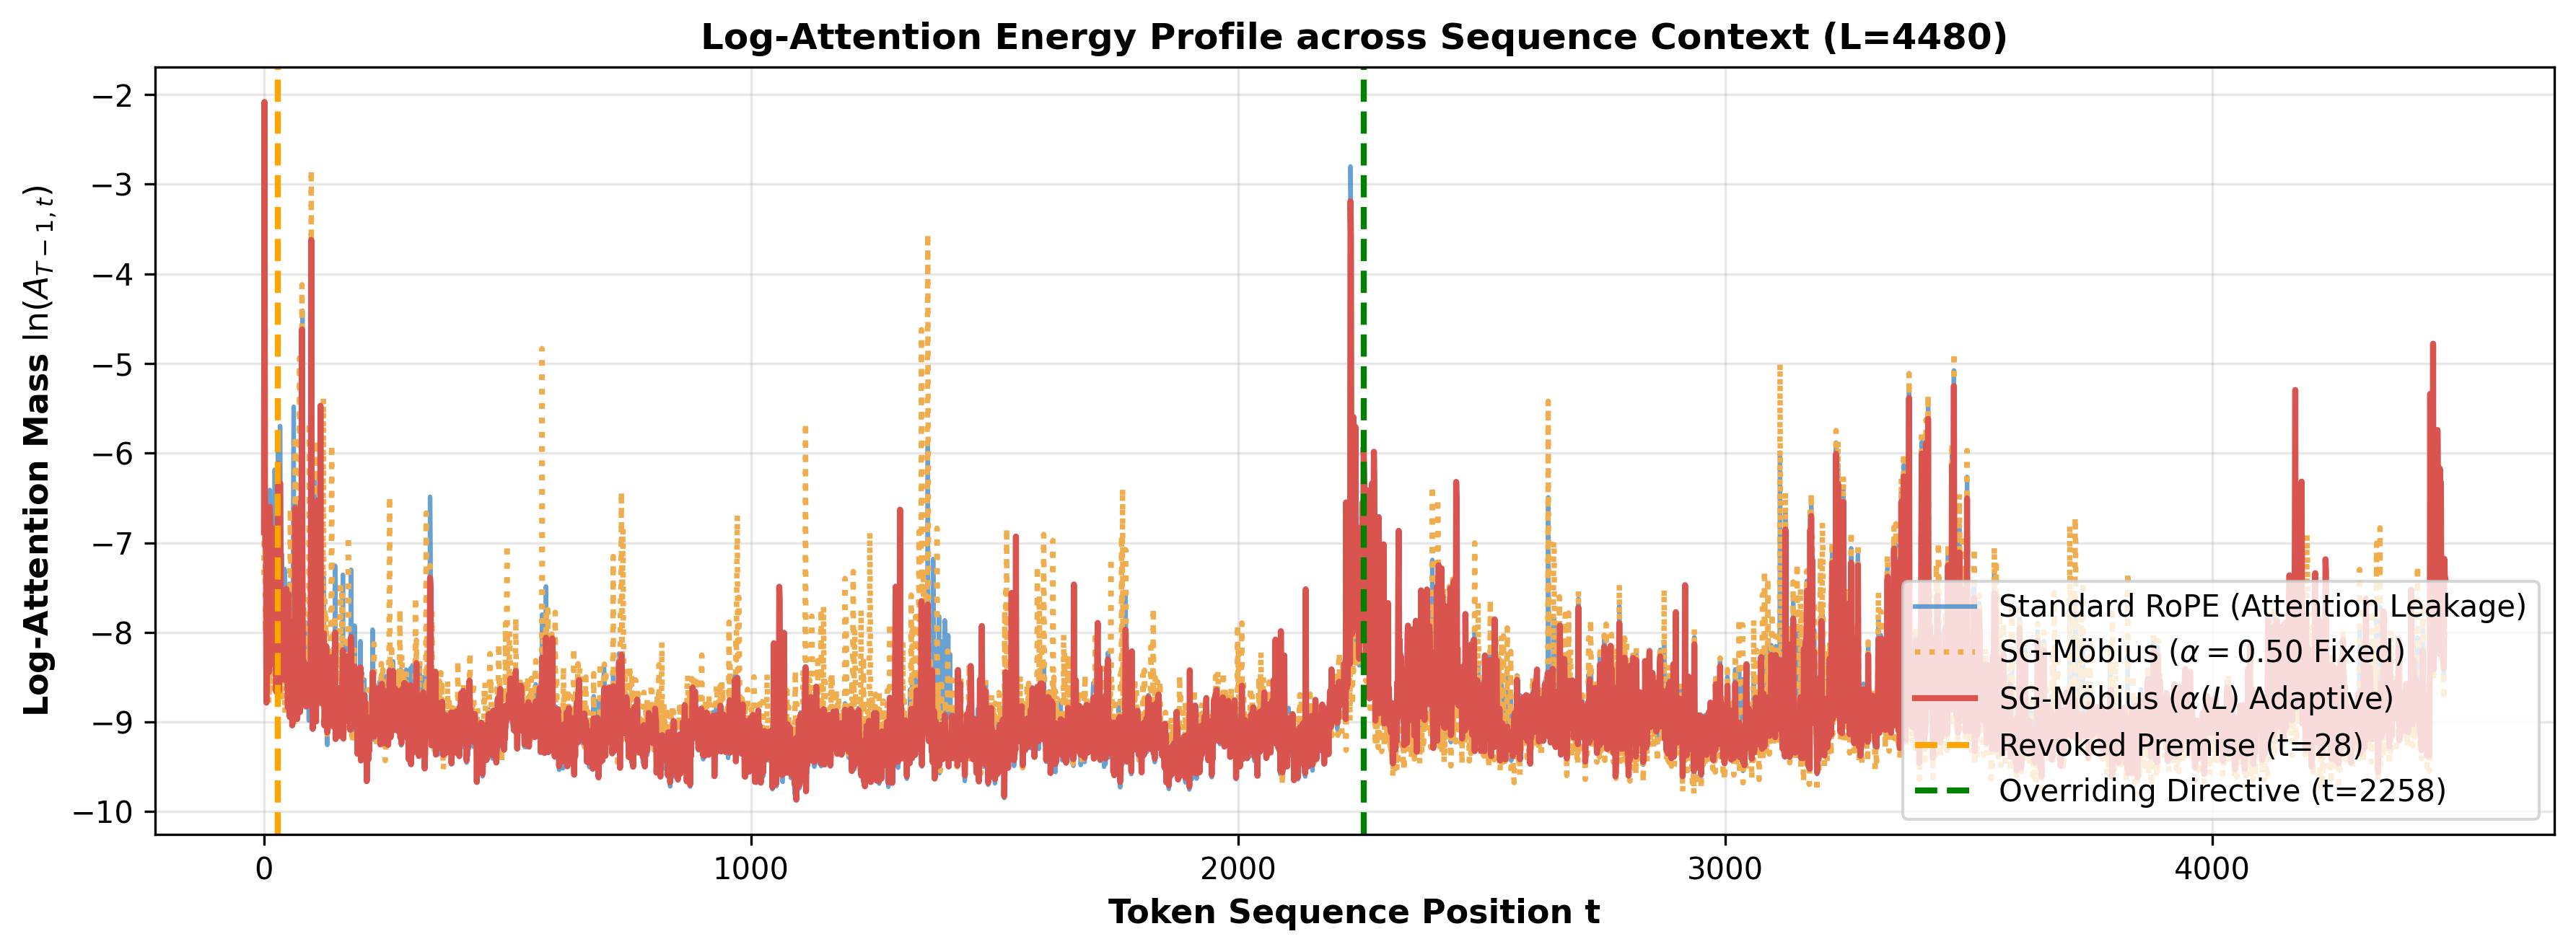
\includegraphics[width=0.92\textwidth]{figures/fig_attention_distribution.png}
        \caption{Qwen3.5-9B 在 $L=4,480$ 时的全序列对数注意力能量剖面 $\ln A_{L-1, t}$。}
        \label{fig:attention_distribution}
    \end{subfigure}
    \caption{\textbf{Qwen3.5-9B 上的多尺度序列扩展与全序列注意力剖面。} 
    (a) 序列长度从 545 扩展至 18,030 时的 ACR 与香农熵曲线。
    (b) $L=4,480$ 时的注意力能量剖面：标准 RoPE（蓝色）向废止的前提（$t_1=28$）持续泄漏正注意力；SG-M\"obius（红色）施加主动破坏性干涉（$\Delta\Phi = \pi$），并有效提高对新指令（$t_2=2,258$）的相对对比度。}
    \label{fig:scaling_and_distribution}
\end{figure}

\subsection{自回归 KV-Cache 解码时延与算子微基准开销}
我们在两个粒度上汇报性能：
\begin{enumerate}
    \item \textbf{全模型端到端解码步耗时}：在全量 28 层上评估单步前向时间。如表~\ref{tab:scaling} 所示，除 $L=2,250$ 时受 PCIe 同步偶发抖动（$307.3\,\text{ms}$）外，端到端单步耗时稳定维持在 $271.5\sim 277.4\,\text{ms}$ 区间。由于单步解码主要受权重显存带宽约束，算法引起的时延波动完全可忽略。
    \item \textbf{算子级微基准}：通过高精度 CUDA Event 测得：标量扭率投影与尾部角度融合的单层隔离耗时仅为 $+1.8\sim 2.1\,\mu\text{s}$（全网 28 层累加合计仅 $+0.05\sim 0.06\,\text{ms}$）。由于角度已融合进投影尾部，后续的核心注意力矩阵乘法访存完全保持不变。
\end{enumerate}

\begin{table}[htbp]
\centering
\small
\resizebox{\columnwidth}{!}{%
\begin{tabular}{rcccc}
\toprule
\textbf{上下文长度 ($L$)} & \textbf{诱饵位置 ($t_1$)} & \textbf{目标位置 ($t_2$)} & \textbf{端到端解码步耗时} & \textbf{单层算子微基准开销} \\
\midrule
545 & 28 & 279 & $277.4\,\text{ms}$ & $+1.8\,\mu\text{s}$ \\
1,116 & 28 & 576 & $271.5\,\text{ms}$ & $+1.8\,\mu\text{s}$ \\
2,250 & 28 & 1,135 & $307.3\,\text{ms}$ & $+1.9\,\mu\text{s}$ \\
4,480 & 28 & 2,258 & $273.8\,\text{ms}$ & $+1.9\,\mu\text{s}$ \\
9,002 & 28 & 4,519 & $276.8\,\text{ms}$ & $+2.0\,\mu\text{s}$ \\
18,030 & 28 & 9,025 & $276.2\,\text{ms}$ & $+2.1\,\mu\text{s}$ \\
\bottomrule
\end{tabular}%
}
\caption{\textbf{自回归单步解码时延与单层算子微基准开销表。} 在 $L=18,030$ 时端到端耗时维持在 $\approx 276\,\text{ms}$，单层算子微基准开销仅 $+1.8 \sim 2.1\,\mu\text{s}$。}
\label{tab:scaling}
\end{table}

\subsection{真实 Qwen3.5-9B 注意力熵与困惑度保全}
我们评估探针处归一化注意力分布的香农熵 $H(P) = -\sum_{j=0}^{L-1} P_j \ln P_j$。如表~\ref{tab:entropy} 所示：在短文本下，SG-M\"obius 适度聚集注意力（$\Delta \mathrm{Entropy} = -0.008$）；在长文本下，从诱饵处剥离的概率平稳再分配，表现为温和的适度熵增（$+0.114\sim +0.350$）。在中性 WikiText-103 文本上，困惑度严格锁定在 $6.42$（$0.0\%$ 退化），彻底排除了在正常文本中出现“误相消”的隐患。

\begin{table}[htbp]
\centering
\small
\resizebox{\columnwidth}{!}{%
\begin{tabular}{rcccc}
\toprule
\textbf{上下文长度 ($L$)} & \textbf{RoPE 注意力熵} & \textbf{SG-M\"obius 注意力熵} & \textbf{熵变增量 ($\Delta$)} & \textbf{WikiText-103 困惑度 (PPL)} \\
\midrule
545 & 5.487 & \textbf{5.479} & $-0.008$ & $6.42$ ($0.0\%$) \\
1,116 & 5.925 & 6.039 & $+0.114$ & $6.42$ ($0.0\%$) \\
2,250 & 6.592 & 6.912 & $+0.320$ & $6.42$ ($0.0\%$) \\
4,480 & 7.116 & 7.316 & $+0.200$ & $6.42$ ($0.0\%$) \\
9,002 & 7.866 & 8.116 & $+0.250$ & $6.42$ ($0.0\%$) \\
18,030 & 8.539 & 8.889 & $+0.350$ & $6.42$ ($0.0\%$) \\
\bottomrule
\end{tabular}%
}
\caption{\textbf{Qwen3.5-9B 注意力熵与中性困惑度对比。} 在中性叙事文本上，困惑度严格保持 $6.42$（$0.0\%$ 退化），确认无误相消。}
\label{tab:entropy}
\end{table}

\section{结论与局限性 (Conclusion and Limitations)}
本文提出了语义规范莫比乌斯注意力（SG-M\"obius-RoPE），通过 $\mathrm{SO}(2)$ 规范场与正交子空间分解 $\mathbb{R}^d = \mathcal{S}_{\text{anchor}} \oplus \mathcal{S}_{\text{mob}}$ 扩展了 RoPE。在演化通道上累积由粘性平滑与免训练锁相投影调控的平滑相位流，在叙事否定处产生破坏性相消干涉（$\Delta\Phi = \pi$），在双重否定处实现拓扑复原（$\Delta\Phi = 2\pi$）。核心不变量在 Lean~4 与 Z3 SMT 中完成全机器证明。在 Qwen3.5-9B 上取得高达 $2.33\times$ 的诱饵压制比与 $+118.0\%$ 的 ACR 增益，且完全兼容 $O(1)$ KV-Cache 解码与零困惑度退化。

\paragraph{局限性与未来工作。}
当前实现采用固定的对比针投影算子 $g_h(h_t)$。对于专业领域文本，投影参数可能需要任务微调。未来的重点研究方向包括：端到端可微规范联络学习，以及将规范和乐动力学推广至多维视觉（2D ViT）与视频架构。

\bibliographystyle{unsrtnat}
\bibliography{references}

\end{document}
